% !TeX encoding = UTF-8
% !TeX program = xelatex
% !TeX spellcheck = en_US

\documentclass[degree=bachelor, fontset=none]{thuthesis}
  % 学位 degree:
  %   doctor | master | bachelor | postdoc
  % 学位类型 degree-type:
  %   academic(默认)| professional
  % 语言 language
  %   chinese(默认)| english
  % 字体库 fontset
  %   windows | mac | fandol | ubuntu
  % 建议终版使用 Windows 平台的字体编译

\setCJKmainfont[AutoFakeBold,ItalicFont=simkai.ttf]{simsun.ttc}
\setCJKfamilyfont{zhkai}[AutoFakeBold]{simkai.ttf}
\setCJKsansfont[AutoFakeBold]{simhei.ttf}
\setCJKfamilyfont{zhsong}[AutoFakeBold]{simsun.ttc}
\setCJKfamilyfont{zhhei}[AutoFakeBold]{simhei.ttf}

% 论文基本配置,加载宏包等全局配置
% !TeX root = ./thuthesis-example.tex

% 论文基本信息配置

\thusetup{
  %******************************
  % 注意:
  %   1. 配置里面不要出现空行
  %   2. 不需要的配置信息可以删除
  %   3. 建议先阅读文档中所有关于选项的说明
  %******************************
  %
  % 输出格式
  %   选择打印版(print)或用于提交的电子版(electronic),前者会插入空白页以便直接双面打印
  %
  output = print,
  %
  % 标题
  %   可使用“\\”命令手动控制换行
  %
  title  = {基于 Cython 的 C++ API 自动包装器设计与实现},
  title* = {An Introduction to \LaTeX{} Thesis Template of Tsinghua
            University v\version},
  %
  % 学位
  %   1. 学术型
  %      - 中文
  %        需注明所属的学科门类,例如:
  %        哲学、经济学、法学、教育学、文学、历史学、理学、工学、农学、医学、
  %        军事学、管理学、艺术学
  %      - 英文
  %        博士:Doctor of Philosophy
  %        硕士:
  %          哲学、文学、历史学、法学、教育学、艺术学门类,公共管理学科
  %          填写“Master of Arts“,其它填写“Master of Science”
  %   2. 专业型
  %      直接填写专业学位的名称,例如:
  %      教育博士、工程硕士等
  %      Doctor of Education, Master of Engineering
  %   3. 本科生不需要填写
  %
  degree-name  = {工学硕士},
  degree-name* = {Master of Science},
  %
  % 培养单位
  %   填写所属院系的全名
  %
  department = {计算机科学与技术系},
  %
  % 学科
  %   1. 学术型学位
  %      获得一级学科授权的学科填写一级学科名称,其他填写二级学科名称
  %   2. 工程硕士
  %      工程领域名称
  %   3. 其他专业型学位
  %      不填写此项
  %   4. 本科生填写专业名称,第二学位论文需标注“(第二学位)”
  %
  discipline  = {计算机科学与技术},
  discipline* = {Computer Science and Technology},
  %
  % 姓名
  %
  author  = {薛瑞尼},
  author* = {Xue Ruini},
  %
  % 指导教师
  %   中文姓名和职称之间以英文逗号“,”分开,下同
  %
  supervisor  = {郑纬民, 教授},
  supervisor* = {Professor Zheng Weimin},
  %
  % 副指导教师
  %
  % associate-supervisor  = {陈文光, 教授},
  % associate-supervisor* = {Professor Chen Wenguang},
  %
  % 联合指导教师
  %
  % co-supervisor  = {某某某, 教授},
  % co-supervisor* = {Professor Mou Moumou},
  %
  % 日期
  %   使用 ISO 格式;默认为当前时间
  %
  % date = {2019-07-07},
  %
  % 是否在中文封面后的空白页生成书脊(默认 false)
  %
  include-spine = true,
  %
  % 密级和年限
  %   秘密, 机密, 绝密
  %
  % secret-level = {秘密},
  % secret-year  = {10},
  %
  % 博士后专有部分
  %
  % clc                = {分类号},
  % udc                = {UDC},
  % id                 = {编号},
  % discipline-level-1 = {计算机科学与技术},  % 流动站(一级学科)名称
  % discipline-level-2 = {系统结构},          % 专业(二级学科)名称
  % start-date         = {2011-07-01},        % 研究工作起始时间
}

% 载入所需的宏包

% 定理类环境宏包
\usepackage{amsthm}
% 也可以使用 ntheorem
% \usepackage[amsmath,thmmarks,hyperref]{ntheorem}

\thusetup{
  %
  % 数学字体
  % math-style = GB,  % GB | ISO | TeX
  math-font  = xits,  % sitx | xits | libertinus
}

% 可以使用 nomencl 生成符号和缩略语说明
% \usepackage{nomencl}
% \makenomenclature


\usepackage[inkscapelatex=false]{svg} % 需使用包

% 表格加脚注
\usepackage{threeparttable}

% 表格中支持跨行
\usepackage{multirow}

% 固定宽度的表格。
% \usepackage{tabularx}

% 跨页表格
\usepackage{longtable}

% 算法
\usepackage{algorithm}
\usepackage{algorithmic}
\renewcommand{\algorithmicrequire}{\textbf{Input:}}
\renewcommand{\algorithmicensure}{\textbf{Output:}}
\newcommand{\code}{\texttt}
% 量和单位
\usepackage{siunitx}

% 代码
\usepackage{listings}
\usepackage{framed}
\lstset{
 columns=fixed,       
%  numbers=left,                                        % 在左侧显示行号
%  numberstyle=\tiny\color{gray},                       % 设定行号格式
 frame=none,                                          % 不显示背景边框
 basicstyle=\ttfamily\footnotesize
}

% 参考文献使用 BibTeX + natbib 宏包
% 顺序编码制
\usepackage[sort]{natbib}
\bibliographystyle{thuthesis-numeric}

% 著者-出版年制
% \usepackage{natbib}
% \bibliographystyle{thuthesis-author-year}

% 本科生参考文献的著录格式
% \usepackage[sort]{natbib}
% \bibliographystyle{thuthesis-bachelor}

% 参考文献使用 BibLaTeX 宏包
% \usepackage[style=thuthesis-numeric]{biblatex}
% \usepackage[style=thuthesis-author-year]{biblatex}
% \usepackage[style=apa]{biblatex}
% \usepackage[style=mla-new]{biblatex}
% 声明 BibLaTeX 的数据库
% \addbibresource{ref/refs.bib}

% 定义所有的图片文件在 figures 子目录下
\graphicspath{{figures/}}

% 数学命令
\makeatletter
\newcommand\dif{%  % 微分符号
  \mathop{}\!%
  \ifthu@math@style@TeX
    d%
  \else
    \mathrm{d}%
  \fi
}
\makeatother

% hyperref 宏包在最后调用
\usepackage{hyperref}



\begin{document}

% 封面
\maketitle

% 学位论文指导小组、公开评阅人和答辩委员会名单
% 本科生不需要
% \input{data/committee}

% 使用授权的说明
\copyrightpage
% 将签字扫描后授权文件 scan-copyright.pdf 替换原始页面
% \copyrightpage[file=scan-copyright.pdf]

\frontmatter
% !TeX root = ../thuthesis-example.tex

% 中英文摘要和关键字

\begin{abstract}
在 Python 语言中调用 C/C++ 跨语言接口是一种常见的需求。Python 语法便捷、应用丰富,C/C++ 性能优越、靠近底层,二者的结合能带来更高的生产力。Cython 语言在 Python 语法的基础上增加了 C 类型标注,能以极低的性能损失封装 C/C++ 接口,是为 Python 构建 C/C++ 扩展模块的理想选择之一。本文设计并实现了一种从 C/C++ 声明中自动构建 Cython 包装模块的开发工具,CPP2PY,以降低学习和编写 Cython 程序的时间成本。CPP2PY 以 C/C++ 头文件为输入,输出构建脚本、 Cython 包装代码和对应的Python 类型标注文件。它经过了详尽的软件测试,支持的语法特性包括全局变量、宏、枚举、类、结构体、联合、继承、重载和类型别名等。基于 CPP2PY,本文封装了 C 算法库 SuiteSparse 实现的大规模稀疏矩阵Cholesky分解算法,为Python科学计算库SciPy实现了正确而高效的稀疏矩阵分解功能。实验表明,封装后的 Python 接口与直接编写C程序相比性能损失低于5\%。

  % 关键词用“英文逗号”分隔,输出时会自动处理为正确的分隔符
  \thusetup{
    keywords = {Cython, 跨语言接口, 自动化构建工具, 稀疏矩阵 Cholesky 分解 },
  }
\end{abstract}

\begin{abstract*}
It is a common requirement to call C/C++ foreign function interfaces in Python.
Python provides convenient syntax and a thriving open source community, while C/C++
is famous for its superior performance and proximity to the underlying layer. The combination of both can lead to higher productivity. The Cython language adds C type annotations to the Python syntax, which can encapsulate C/C++ interfaces with little performance losses, making it an ideal choice for building C/C++ extension modules for Python. This article designed and implemented a development tool, CPP2PY, that automatically builds Cython wrappers from C/C++ declarations to reduce the cost of learning and writing Cython programs. CPP2PY takes C/C++ header files as input and outputs setup scripts, Cython wrapping codes, and corresponding Python type annotation files. It has undergone sufficient testing and supports syntax features such as global variables, macros, enumerations, classes, structs, unions, inheritance, overloading, type aliases, etc. Based on CPP2PY, we encapsulated the Cholesky decomposition algorithm for large-scale sparse matrixes implemented by SuiteSparse, a C algorithm library, to achieve a correct and efficient sparse matrix decomposition function for Python scientific computing library SciPy. Experiments have shown that the performance loss of the Python interface is less
than 5\% compared to writing C programs directly.

  % Use comma as separator when inputting
  \thusetup{
    keywords* = {Cython, FFI, Automated Build Tool, Sparse Cholesky Decomposition},
  }
\end{abstract*}


% 目录
\tableofcontents

% 符号对照表
% !TeX root = ../thuthesis-example.tex

\begin{denotation}[3cm]
  \item[API] 应用程序接口
  \item[IDE] 集成开发环境
  \item[FFI] 跨语言函数接口
  \item[AST] 抽象语法树
  \item[getter] 读访问器
  \item[setter] 写访问器
\end{denotation}



% 也可以使用 nomencl 宏包,需要在导言区
% \usepackage{nomencl}
% \makenomenclature

% 在这里输出符号说明
% \printnomenclature[3cm]

% 在正文中的任意为都可以标题
% \nomenclature{PI}{聚酰亚胺}
% \nomenclature{MPI}{聚酰亚胺模型化合物,N-苯基邻苯酰亚胺}
% \nomenclature{PBI}{聚苯并咪唑}
% \nomenclature{MPBI}{聚苯并咪唑模型化合物,N-苯基苯并咪唑}
% \nomenclature{PY}{聚吡咙}
% \nomenclature{PMDA-BDA}{均苯四酸二酐与联苯四胺合成的聚吡咙薄膜}
% \nomenclature{MPY}{聚吡咙模型化合物}
% \nomenclature{As-PPT}{聚苯基不对称三嗪}
% \nomenclature{MAsPPT}{聚苯基不对称三嗪单模型化合物,3,5,6-三苯基-1,2,4-三嗪}
% \nomenclature{DMAsPPT}{聚苯基不对称三嗪双模型化合物(水解实验模型化合物)}
% \nomenclature{S-PPT}{聚苯基对称三嗪}
% \nomenclature{MSPPT}{聚苯基对称三嗪模型化合物,2,4,6-三苯基-1,3,5-三嗪}
% \nomenclature{PPQ}{聚苯基喹噁啉}
% \nomenclature{MPPQ}{聚苯基喹噁啉模型化合物,3,4-二苯基苯并二嗪}
% \nomenclature{HMPI}{聚酰亚胺模型化合物的质子化产物}
% \nomenclature{HMPY}{聚吡咙模型化合物的质子化产物}
% \nomenclature{HMPBI}{聚苯并咪唑模型化合物的质子化产物}
% \nomenclature{HMAsPPT}{聚苯基不对称三嗪模型化合物的质子化产物}
% \nomenclature{HMSPPT}{聚苯基对称三嗪模型化合物的质子化产物}
% \nomenclature{HMPPQ}{聚苯基喹噁啉模型化合物的质子化产物}
% \nomenclature{PDT}{热分解温度}
% \nomenclature{HPLC}{高效液相色谱(High Performance Liquid Chromatography)}
% \nomenclature{HPCE}{高效毛细管电泳色谱(High Performance Capillary lectrophoresis)}
% \nomenclature{LC-MS}{液相色谱-质谱联用(Liquid chromatography-Mass Spectrum)}
% \nomenclature{TIC}{总离子浓度(Total Ion Content)}
% \nomenclature{\textit{ab initio}}{基于第一原理的量子化学计算方法,常称从头算法}
% \nomenclature{DFT}{密度泛函理论(Density Functional Theory)}
% \nomenclature{$E_a$}{化学反应的活化能(Activation Energy)}
% \nomenclature{ZPE}{零点振动能(Zero Vibration Energy)}
% \nomenclature{PES}{势能面(Potential Energy Surface)}
% \nomenclature{TS}{过渡态(Transition State)}
% \nomenclature{TST}{过渡态理论(Transition State Theory)}
% \nomenclature{$\increment G^\neq$}{活化自由能(Activation Free Energy)}
% \nomenclature{$\kappa$}{传输系数(Transmission Coefficient)}
% \nomenclature{IRC}{内禀反应坐标(Intrinsic Reaction Coordinates)}
% \nomenclature{$\nu_i$}{虚频(Imaginary Frequency)}
% \nomenclature{ONIOM}{分层算法(Our own N-layered Integrated molecular Orbital and molecular Mechanics)}
% \nomenclature{SCF}{自洽场(Self-Consistent Field)}
% \nomenclature{SCRF}{自洽反应场(Self-Consistent Reaction Field)}



% 正文部分
\mainmatter
% !TeX root = ../thuthesis-example.tex

\chapter{绪论}

\section{项目背景}

CPP2PY \cite{bestoftwo}是一个基于 Cython 的软件开发工具,用于简化为 C/C++ 程序编写 Python 接口的工作。本质上说,CPP2PY 是一个编译器,以 C/C++ 声明为输入,创建从 Python 语言调用这些声明所需的包装器。利用CPP2PY,使用者通常可以在几分钟内为小型 C/C++ 项目建立可用的 Python 接口,而不需要修改现有代码。该工程的可能应用包括:

\begin{itemize}
    \item 使用 Python 脚本或交互式命令行(IDLE 或 Jupyter notebook)测试 C/C++ 程序;
    \item 为 C/C++ 程序开发图形化的用户界面,如基于 Flask、Django 等 Python Web 框架;
    \item 为 Python 建立高性能的 C/C++ 模块;
    \item 快速原型设计。
\end{itemize}

为了说明本项目的潜力,有必要列举 C/C++ 编程的优势和痛点,让我们先从前者开始:

\begin{itemize}
    \item 性能优越;
    \item 系统级编程,比如在 C 语言中内嵌汇编指令;
    \item C++ 强大的抽象能力;
    \item 高度优化的编译器,分布广泛的用户社区和数不清的历史遗产。
\end{itemize}

总而言之,很多时候,C/C++ 都是不可替代的,这使得开发者不得不忍受 C/C++ 编程中的如下问题:

\begin{itemize}
    \item 编写用户界面并不容易;
    \item 软件测试的大量时间耗费在编译-调试循环中;
    \item 模块化机制复杂,缺乏通用包管理器,难以二次开发;
    \item 各种安全问题,如缓存区溢出等。
\end{itemize}

作为对比,在 Python 这样的脚本语言中,编写一个图形用户界面要容易得多;交互式的解释器也可能成为有用的调试和测试工具;数目庞大的第三方库可供选择,诸如 pip,conda 这样的包管理器让调用他人的代码简单又自然;开发者通常不必担心内存泄露问题,有自动垃圾回收器保驾护航……任何编程语言都不可能是完美的,但不同的编程语言提供了不同的优势。

当 Python 被用来控制 C/C++ 程序时,产生的系统往往如图 1 所示。在这种编程模型中,开发者使用 Python 语言驾驭较高的抽象层级,利用特定的脚本指令访问 C/C++ 程序的底层功能。这种双语言编程模式是非常强大的,因为它利用了每种语言的优势:C/C++ 能带来高效的性能,处理复杂的系统编程任务;Python 能提供快速原型设计、交互式调试和方便的高级数据结构。

通过将 Python 和 C/C++ 结合在一起,开发者可以充分利用二者的特点,大大简化软件开发的某些方面。将 C/C++ 整合到 Python 语言中,往往会带来更好的模块化设计、更少的代码、更大的灵活度、以及更高的生产力。

\begin{figure}
  \centering
  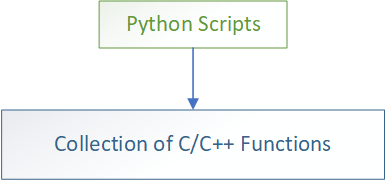
\includegraphics[width=0.5\linewidth]{figures/双语模型.png}
  \caption{Python - C/C++ 双语言编程模型}
  \label{fig:1}
\end{figure}

CPP2PY 最初是为了封装 C 稀疏矩阵算法库 SuiteSparse 中的稀疏分解算法而编写的。它以 libclang 为编译前端,Cython 为编译后端,解析 C/C++ 头文件生成 Cython 代码、构建文件和相应的 Python 存根文件。本项目在设计上避免生成过于复杂的代码,使用者可以方便地在生成结果的基础上进行二次开发。得益于 Cython,借助 CPP2PY 为 Python 编写 C/C++ 跨语言接口往往能享受高性能和良好的可扩展性。

\section{Python 的 C/C++ 扩展}

作为脚本语言,Python 的核心是 Python 解释器,也就是 CPython。解释器控制着 Python 脚本的执行和变量的访问。通过扩展解释器,可以添加新的命令和变量。CPython 提供了用于定义这种新命令的特殊接口,规定了这些新命令应该如何与解释器挂钩,这就是 CPython C API\cite{pyc}。

为了将新的 C/C++ 接口嵌入 CPython 中,需要编写一个特殊的包装函数,充当 Python 解释器与底层接口之间的粘合剂;然后向Python 解释器提供包装函数的名称、参数等信息。然而,直接以这种方式创建扩展模块费时费力,Python 官方文档建议, 尽可能使用第三方工具,如 Cython,SWIG,cffi 等,以更简单、更精致的方式为 Python 构建 C/C++ 扩展\footnote{“Third party tools like Cython, cffi, SWIG and Numba offer both simpler and more sophisticated approaches to creating C and C++ extensions for Python.”}。

\subsection{Cython}

作为本项目的起点,Cython 将在本文中多次出现。它包含两重含义,Cython 语言和 Cython 编译器。

Cython 语言\cite{O2015Cython, cython} 保留了 Python 的大部分语法,但额外支持调用 C 函数,支持为变量和类成员声明 C 类型。Cython 编译器将 Cython 代码编译为 C/C++ 代码,C/C++ 编译器再将这些代码编译为二进制形式的 Python 模块。以这种形式生成的扩展充分利用了静态类型信息,在性能上高度优化,与相应 C 程序相差无几。

除了高性能之外,Cython 的其它优势包括内置 Numpy C API、无运行时依赖等。作为编写高性能子模块的不二之选,Cython 被应用在 Python 数值计算、数据处理、机器学习等领域,著名第三方库如 scipy、pandas、sklearn 中都有它的身影。

作为一门小众语言,Cython 也存在一些缺陷,主要包括:

\begin{itemize}
    \item 缺少 IDE 支持,缺乏代码高亮、自动补全、自动格式化等开发工具;
    \item 作为一门语言来说,缺少系统完善的文档;
    \item 缺乏对 C++ 高级特性的支持。
\end{itemize}

CPP2PY 将 Cython 程序编写中的大部分任务自动化,能有效缓解其文档、辅助开发工具不足带来的不便。具体来说,利用 Cython 为 C/C++ 程序编写 Python 接口,通常需要三个步骤:

\begin{itemize}
    \item [1)] 罗列需要的 C/C++ 接口声明;
    \item [2)] 编写调用接口所需的 Cython 代码,根据需求进行扩展;
    \item [3)] 编写构建脚本,指定编译、链接参数。
\end{itemize}

这之中包含大量简单重复的工作,CPP2PY 正为此而生,它自动解析 C++ 头文件,生成接口声明和对应的包装代码,并自动生成构建脚本。

\subsection{与替代选择的比较}

除了 Cython 之外,还有其他第三方工具能为 C/C++ 程序编写 Python 接口,表 \ref{tab:1.2} 罗列了它们各自的特色\cite{msdnexperiment, cythonothers}。

\begin{table}
  \centering
  \caption{在 Python 中编写 C/C++ 扩展的可选方法}
  \begin{tabular}{lll}
    \toprule
     方法      &  创建年份  &  特色                           \\
    \midrule
     Cython    &  2007      &  高性能、NumPy 交互             \\
     PyBind11  &  2015      &  支持更多 C++ 高级特性          \\
     SWIG      &  1996      &  支持除 Python 外的其它目标语言 \\
     ctype     &  2003      &  Python 标准库                  \\
     cffi      &  2013      &  ctype 的替代选择,在运行时动态提供跨语言接口         \\
    \bottomrule
  \end{tabular}
  \label{tab:1.2}
\end{table}



其中,ctype 和 cffi 只支持 C 语言;PyBind11 和 SWIG\cite{swig} 要求开发者编写 C++ 代码指定封装的细节。而 Cython 与其它专为编写跨语言接口而生的竞争者不同,它是一门完整的编程语言,具有更强的可扩展性。

表 \ref{tab:1.3} 比较了支持 C++ 的各种第三方工具的性能。测试的方法是以各种工具包装用 C++ 编写的双曲正切函数 
\begin{equation}
    tanh(x) = \frac{e^x-e^{-x}}{e^x+e^{-x}}
\end{equation}
随机生成一千万个均匀分布于 $(-2,2)$ 之间的浮点数,通过跨语言接口计算其双曲正切函数值。由测试结果可知,Cython 在性能方面尤为突出,与直接使用 CPython C API 相差无几。

\begin{table}
  \centering
  \caption{不同扩展方式的性能比较}
  \begin{tabular}{ll}
    \toprule
     方法           &  用时 (s) \\
    \midrule
     纯 Python      &  4.939    \\
     CPython C API  &  1.210    \\
     Cython         &  1.254    \\
     PyBind11       &  2.464    \\
     SWIG           &  2.000    \\
    \bottomrule
  \end{tabular}
  \label{tab:1.3}
\end{table}

综合考虑各个工具的特点,可以得出以下结论:如果开发者对跨语言接口的性能有较高要求,或者希望利用 Numpy C API,应选择 Cython 作为开发工具;而如果希望尽可能保留 C++ 语言的高级特性,则可选用 PyBind11;如果需要在项目中使用第三种语言,则可选择 SWIG。值得一提的是,如果开发者只想加速 Python 代码,而不是封装已有的 C/C++ 程序,则应该先尝试 Numba,它为 Python 语言的一个子集和 NumPy 提供了 CPU 和 GPU 上的自动并行功能。

\section{相关工作}

Cython 百科\footnote{\url{https://github.com/cython/cython/wiki/AutoPxd}}列举了一些已有的且仍在维护中的同类型工具,包括 python-autopxd 和 autowrap,前者解析 C 头文件生成 Cython 声明,后者解析 Cython 声明生成包装代码。然而,本文的工作并未参考它们,从功能上说,本项目支持解析 C++ 语法,并能同时生成 Cython 声明和包装代码,与已有工具相比更加全面。

要将 C++ 程序迁移到 Python 中 会面临许多困难。首先,C++ 语法极为复杂,CPP2PY 依靠 libclang 来处理 C++ 头文件、分析类型系统;另外,C++ 与 Python 在很多方面有根本性的差异,许多 C++ 语法在 Python 或 Cython 中没有对应,CPP2PY 不得不采用一些折衷的方式处理它们。本文主要参考了 SWIG\cite{swig} (Simplified Wrapper and Interface Generator)对全局变量、类和重载的处理,详见第二章与第三章。CPP2PY 与 SWIG 的本质区别在于编译目标不同——CPP2PY 生成 Cython 代码,而SWIG 直接生成 C/C++ 代码。

\section{本文结构与贡献}

本文分为五个章节,第一章为绪论,介绍项目背景、技术路线和相关工作。

第二章介绍关键部分的设计、模块划分,以及软件测试情况。

第三章详细介绍了本程序的功能和使用方法。

第四章以稀疏矩阵库 SuiteSparse 中的稀疏矩阵 Cholesky 分解算法为例,介绍本项目的应用。

第五章为总结。

截至目前,CPP2PY 支持的特性包括:

\begin{itemize}
    \item 全局变量和宏;
    \item 基本数据类型及其指针、数组,部分 STL 容器;
    \item 枚举、联合、结构体与类;
    \item 类的静态成员、继承、运算符重载、抽象类;
    \item 默认参数、类型别名、异常、命名空间等;
    \item 生成对应 Python 存根文件,为二进制模块提供代码补全和类型注解。
\end{itemize}

所有这些特性及其限制将在第三章详细说明。本项目所有代码托管于 \url{https://github.com/zhanghx0905/cpp2py-cython}。 
% !TeX root = ../thuthesis-example.tex

\chapter{程序设计}

\section{从 C++ 到 Python}

\subsection{包装函数}
一个 Cython 包装函数分为三部分:

\begin{itemize}
    \item 将输入的 Python 对象转换为特定类型的 C++ 变量;
    \item 调用 C/C++ 接口,传入转换后的输入参数;
    \item 将接口的返回值转换为 Python 对象。
\end{itemize}

Cython 能自动处理一部分 C/C++ 类型与 Python 对象间的类型转换,包括基本数值类型、字符串和部分 STL 容器。对于其它类型,包括数组、指针、枚举、类、结构体和联合,CPP2PY 为其专门生成类型转换代码。函数和类方法都以这种方式得到包装。

类的数据成员在 Python 侧被包装为类的属性,CPP2PY 专门为其生成 getter 函数,如果该数据成员或变量是可变的,还会生成 setter 函数。例如,对于如下 C++ 声明,
\begin{framed}
\begin{lstlisting}[language=c++]
struct Point {
    int x;
    const char * LUCKY;
}
\end{lstlisting}
\end{framed}将生成对应 Python 接口,

\begin{framed}
\begin{lstlisting}[language=Python]
class Point:
    @property
    def x(self) -> np.int32: ...
    @x.setter
    def x(self, x: np.int32): ...
    @property
    def LUCKY(self) -> str: ...
\end{lstlisting}
\end{framed}
容易看出,getter 是参数为空,返回值类型为对应变量类型的方法,而 setter 的返回值为空,唯一的参数类型为相应变量类型。生成它们的逻辑与普通的函数或方法完全一致。

CPP2PY 支持 C/C++ 的全局变量,然而,背后的实现机制并不直观。当你在 Python 中写下这段代码时,

\begin{framed}
\begin{lstlisting}[language=python]
pi = 3.14
a = pi
\end{lstlisting}
\end{framed}

\noindent 只有一个对象包含浮点数 3.14,而 \lstinline{a} 和 \lstinline{pi} 都是它的名称。这种赋值机制与 C/C++ 完全不同——对于后者来说,一个变量指向一段内存,赋值表示将数据复制到该内存位置。因此,没有直接的方法将 C 中的变量赋值映射到 Python 中的变量赋值。CPP2PY 处理全局变量的方法是创建一个特殊的全局对象,将全局变量包装为该对象的属性。

这样,CPP2PY 以一种优雅的方式统一封装了变量、函数、方法和数据成员。

\subsection{代理类}

Cython 提供了两种定义类的语法,一种是普通的 Python 类,另一种被称为扩展类。与 Python 类相比,扩展类使用 C 结构体,而不是 Python 字典来存储字段和方法,因而具有显著的性能优势。扩展类中可以存储 C 类型字段,CPP2PY 用它来封装类、结构体与联合。

CPP2PY 在 Cython 端为 C++ 类生成代理类,即同名的 Python 扩展类,其中保存了指向 C++ 对象的指针和标记指针所有权的布尔属性,在构造函数中分配内存并获取所有权,在析构函数中检查所有权、释放内存。代理类机制使得 Python 用户能以非常自然的方式访问 C++ 数据结构。

\begin{framed}
\begin{lstlisting}[language=Python]
def __cinit__(self):
    self.thisptr = NULL
    self.owner = True

def __dealloc__(self):
    if self.owner and self.thisptr != NULL:
        del self.thisptr
        self.thisptr = NULL
\end{lstlisting}
\end{framed}

美中不足的是,与普通 Python 类相比,扩展类只支持有限的面向对象语法。类的静态数据成员不受支持,CPP2PY 将它们视作带作用域的变量;扩展类间的多重继承不受支持,也不允许在子类中重定义 C 类型字段。CPP2PY 以一种间接的方式处理继承——拷贝超类所有的方法和数据成员到派生类中。这种实现的优点是避免生成过于复杂的代码,也支持了多重继承,而缺点则是,类的继承关系将无法从 C++ 映射到 Python 中,第三章中详细阐述了这种妥协带来的限制。

为了计算出一个类所有的超类和派生类,CPP2PY 根据类的继承关系做拓扑排序。

\begin{figure}
  \centering
  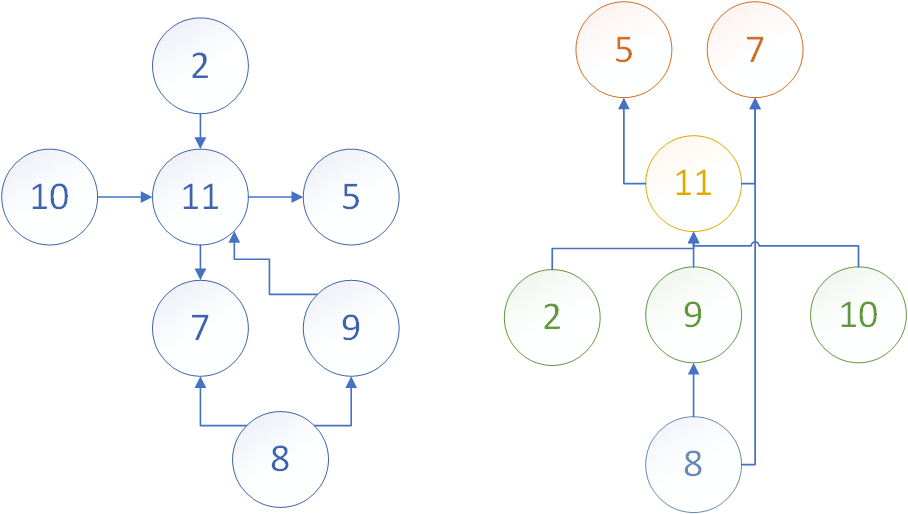
\includegraphics[width=0.8\linewidth]{figures/拓扑排序.png}
  \caption{拓扑排序前后的复杂继承关系图}
  \label{fig:2.4}
\end{figure}

为了说明拓扑排序的效果,考虑如图 \ref{fig:2.4} 左侧所示的复杂继承关系,图中每个节点都代表一个类,每条边由子类指向它的父类,在左图中想要找到类 8 所有的超类并不容易。根据类的父子关系对它们拓扑排序后,得到的结果如图 3 右侧所示。可以立即看出,类 11 依赖于类 5 和类 7,而类 8 依赖于类 9、类11,类 5 和类 7。类 5 和类 7 的拓扑序最靠前,而类 11 次之,类 8 的拓扑序排在最后,一个类的超类在拓扑序列必定排在它前面,派生类必定排在后面。

得到拓扑序后,只需按顺序逐个将每个类的所有父类接口拷贝到类中,即可完成拷贝超类接口的任务。

\section{模块设计}

\begin{figure}
  \centering
  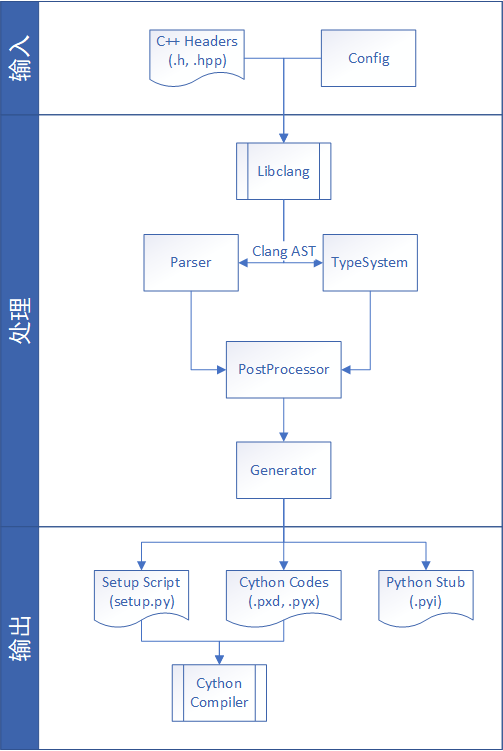
\includegraphics[width=\linewidth]{figures/程序结构.png}
  \caption{模块划分与数据流图}
  \label{fig:2}
\end{figure}

CPP2PY 以 Python 语言编写,其模块设计如图 \ref{fig:2} 所示。程序主要包含五个子模块,分别是 Config、Parser、TypeSystem、PostProcessor 和 Generator;此外还依赖于两个外部库,用于解析 C++ 代码的 libclang 和用于编译目标代码的 Cython。

Config 模块定义了控制程序行为的输入参数,libclang 负责解析 C++ 头文件,生成源文件的抽象语法树 (Abstract Syntax Tree)。Parser 模块解析抽象语法树,从中提取所有必要信息,作为 PostProcessor 的输入。

TypeSystem 建立在 libclang 的类型系统之上。该模块还定义了在 C++ 和 Python 之间转换数据的类型转换器,并对相当一部分类型内置了转换功能。通过继承类型转换器抽象类,用户可以重新定义类型转换的行为,或者使 CPP2PY 支持新的数据类型。

PostProcessor 模块接受 Parser 模块的输入,处理类的继承、函数重载等问题,并为函数、方法和变量绑定类型转换器。

Generator 接受  PostProcessor 的输入,输出目标代码。 生成的文件包括 Cython 代码、Python 构建脚本和存根。

其中, Cython 代码文件分成两部分,所有 C++ 接口的声明在 Cython 声明文件(\lstinline{.pxd})中,而 Cython 实现文件(\lstinline{.pyx})包含了封装这些接口的代码。这样设计使得 C++ 接口与 Python 接口不在同一个作用域内,避免了名称冲突,也给用户二次开发提供了更多的便利。

Python 存根文件与普通 Python 文件的区别是不包含具体实现。利用它,Python IDE 就能为 CPP2PY 生成的二进制代码库提供类型注解和代码补全。得益于此,用户的开发体验将大大提高。不过值得一提的是,作为动态类型语言,Python 并不在乎对象的实际类型,而只关心它是否实现了特定的属性或方法。这种类型系统通常被称为“鸭子类型”。

构建脚本指明了目标代码编译、链接的参数,用户可以根据自己的需要修改构建脚本。虽然 CPP2PY 只在 Ubuntu 上进行了测试,但得益于 Python 构建工具 setuptools,它生成的代码能方便地在不同平台上编译,达到“一次生成,处处构建”的效果。

\section{基于 libclang 的 C++ 头文件解析}

众所周知,C++ 的语法复杂多变,包含了数种编程范式,不计其数的边界情况和庞大的历史包袱。Clang 是 LLVM 的编译前端,支持 C、C++、Objective-C 三种语言的解析。libclang\cite{libclang} 提供了访问 Clang 抽象语法树的 Python 接口,CPP2PY 依赖它完成 C++ 语法解析任务。

Clang 抽象语法树的组成如图 \ref{fig:2.2} 所示,根节点可视为顶层命名空间,它的子节点类型包括命名空间、枚举、类、结构体、联合、变量、函数、类型别名和宏;而类节点的子节点类型又包括数据成员、静态数据成员、方法、构造函数等……根据这样的父子节点关系,Parser 模块层层迭代遍历抽象语法树。

\begin{figure}
  \centering
  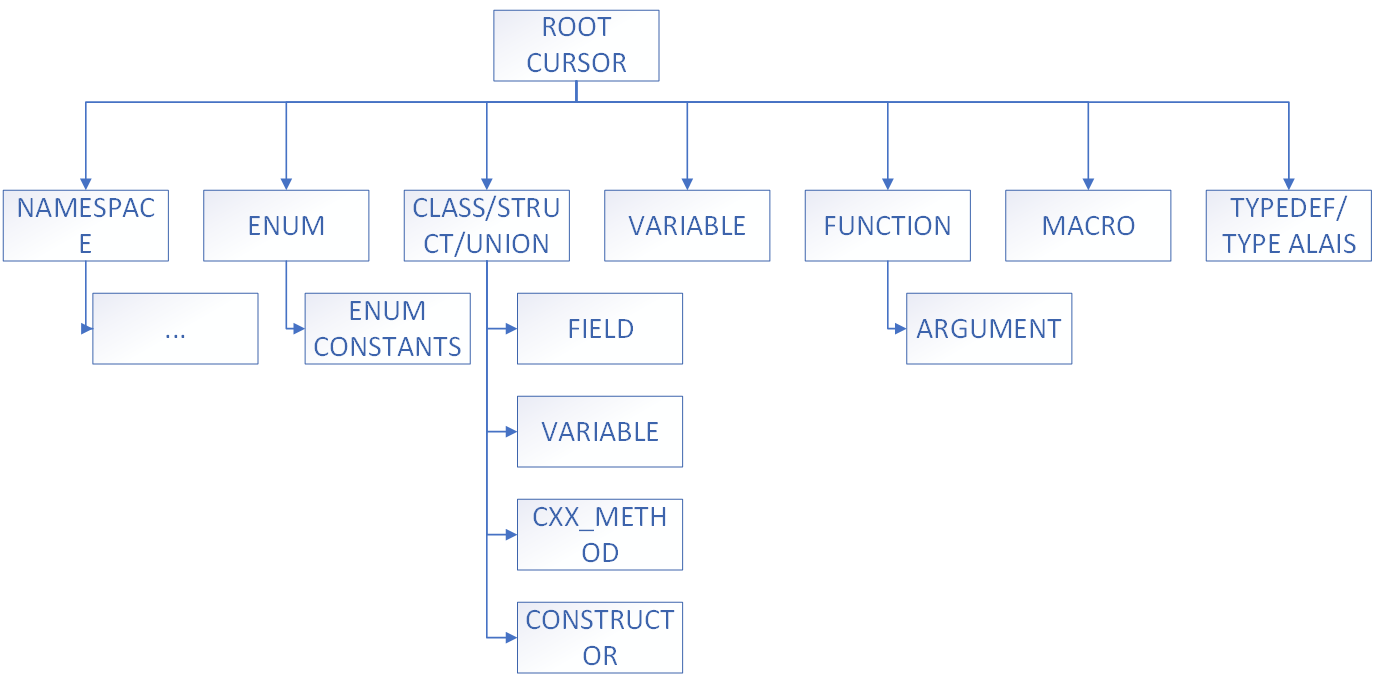
\includegraphics[width=\linewidth]{figures/ClangAST.png}
  \caption{Clang 抽象语法树示意图}
  \label{fig:2.2}
\end{figure}

在解析过程中,C++ 的结构体和联合可以被视作特殊的类,它们的独特之处仅仅在于结构体的成员和继承方式默认为公有,而类默认为私有;联合的所有数据成员共用同一块内存。同样的道理,通过不同语法定义的类型别名也没有实质上的差别。在 C++ 中,通过类的对象访问其非公有成员是不可能的,因此类的任何非公有成员都将被忽略。

解析宏是一件困难的事,因为宏不带有任何额外的类型信息。一个宏可能定义了一段过程、一个类型别名、也可能递归生成了非常复杂的代码。CPP2PY 只能识别定义了简单字面量的宏,包括数值类型和字符串,忽略它解析不了的宏定义。


\section{软件测试}

\begin{figure}
  \centering
  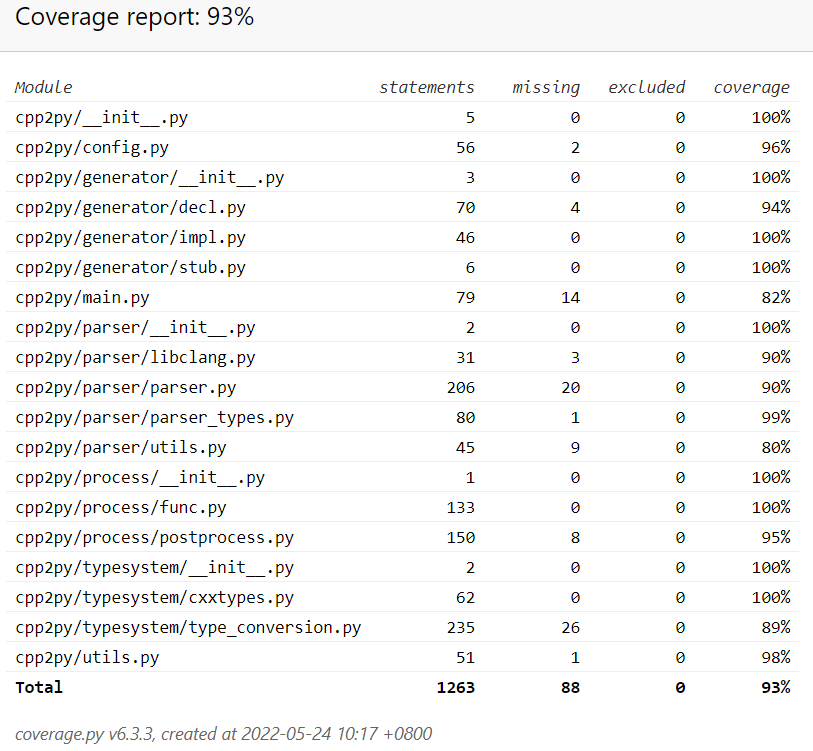
\includegraphics[width=\linewidth]{figures/测试覆盖.png}
  \caption{软件测试覆盖率}
  \label{fig:2.5}
\end{figure}

合理的软件测试既能保证程序的正确运行,又能提高设计和开发的生产力。CPP2PY 的测例分单元测试和集成测试两类。单元测试主要测试程序的功能性模块,如拓扑排序、宏文本解析等。而集成测试以 C++ 代码为输入,测试 CPP2PY 能否正确地解析输入、生成目标代码并编译运行、实现预期的封装效果。

CPP2PY 经过了充分的测试,代码覆盖率达 93\%,如图 \ref{fig:2.5} 所示。测试环境为 Ubuntu 20.04,软件版本为 Python 3.8.10、Cython 0.29.28、libclang 12。

% !TeX root = ../thuthesis-example.tex

\chapter{功能介绍}

\section{运行 CPP2PY}

CPP2PY 能以命令行工具和 Python API 两种方式运行,其主要输入参数如表 \ref{tab:3.1} 所示。这些输入参数可分为四类,指定输入输出文件信息的基本参数、传递给 Libclang 的输入解析参数、传递给构建脚本的编译参数、以及控制代码生成行为的其它参数。其中前三类参数的语义大多是显而易见的,第四类参数将在下文中介绍。

\begin{table}
  \centering
  \caption{CPP2PY 的主要输入参数}
  \begin{tabular}{lll}
    \toprule
     参数名                 &  参数解释                                  &  默认值   \\
    \midrule
     \lstinline$headers$                &  C++ 头文件路径                            &  -        \\
     \lstinline$sources$                &  C++ 实现文件路径                          &  空       \\
     \lstinline$modulename$             &  生成模块名                                &  -        \\
     \lstinline$setup_filename$         &  生成的构建脚本名                          &  setup.py \\
     \lstinline$target$                 &  生成文件路径                              &  当前路径 \\
     \lstinline$encoding$               &  文件编码                                  &  UTF8     \\
     \lstinline$incdirs$                &  Libclang 头文件包含路径                   &  空       \\
     \lstinline$libclang_flags$         &  传递给 Libclang 的额外参数,如 \lstinline$-DDEBUG$  &  空       \\
     \lstinline$libraries$              &  外部链接库                                &  空       \\
     \lstinline$library_dirs$           &  外部链接库路径                            &  空       \\
     \lstinline$compiler_flags$         &  编译选项                                  &  空       \\
     \lstinline$build$                  &  是否编译 Cython 代码                      &  \lstinline$True$     \\
     \lstinline$generate_stub$          &  是否生成 Python 存根文件 (.pyi)           &  \lstinline$True$     \\
     \lstinline$global_vars$            &  全局变量和宏所在对象名                    &  \lstinline$cvar$     \\
     \lstinline$registered_converters$  &  自定义的类型转换器                        &  空       \\
     \lstinline$renames_dict$           &  自定义的函数和变量重命名规则              &  空       \\
    \bottomrule
  \end{tabular}
  \label{tab:3.1}
\end{table}

通过命令行指令调用 CPP2PY,是打包简单 C/C++ 程序的不二之选。例如,下列指令将由头文件 modules.h 和代码文件 modules.cpp 组成的 C++ 项目打包成 Python 包,并命名为 cppproj。

\begin{framed}
\begin{lstlisting}[language=sh]
cpp2py modules.h --sources modules.cpp --modname cppproj
\end{lstlisting}
\end{framed}

如果有较为复杂的需求,如链接已有的动态共享库,则可以编写 Python 脚本,通过 API 调用 CPP2PY。下例指定了动态共享库的路径,如果不这样做的话,将在运行时因找不到共享库而引发导入异常。

\begin{framed}
\begin{lstlisting}[language=python]
from cpp2py import Config, make_cython_extention

config = Config(
    # ...
    library_dirs=[library_dir]
)
make_cython_extention(config)
\end{lstlisting}
\end{framed}

\section{函数}

当类型转换器模块提供了所有参数和返回值的处理方法时,C/C++ 函数被包装为 Python 函数。默认情况下,CPP2PY 支持的数据类型如表 \ref{tab:3.2} 所示。

\begin{table}
  \centering
  \begin{threeparttable}[c]
  \caption{数据在 C++ 与 Python 间的转换}
  \label{tab:3.2}
  \begin{tabular}{p{120pt}p{200pt}p{100pt}}
    \toprule
     Python =>                   &  C++                                                           &  => Python                 \\
    \midrule
     -                           &  \lstinline$void$                                                          &  \lstinline$None$                      \\
     基本数值类型   &  基本数值类型,包括布尔、整数、浮点、复数(\lstinline$std::complex$)  & 基本数值类型 \\
     \lstinline$array.array$, \lstinline$numpy.ndarray$  &  基本数值类型指针                                            &  被指向的数据              \\
     \lstinline$Iterable$                    &  基本数值类型定长数组                                        &  \lstinline$list$                      \\
     \lstinline$str$                         &  字符串(\lstinline$char *$, \lstinline$std::string$)                                 &  \lstinline$str$                      \\
     \lstinline$Iterable[str]$               &  字符数组(\lstinline$char **$)                                           &  被指向的字符串            \\
     \lstinline$Mapping$/\lstinline$Iterable$            &  STL 容器\tnote{①}  & \lstinline$set$/\lstinline$list$/\lstinline$dict$/\lstinline$tuple$    \\
     枚举类                      &  枚举                                                          &  枚举类                    \\
     类                          &  类、结构体、联合\tnote{②}                            &  类                        \\
     类                          &  类、结构体、联合的指针和二重指针                                    &  类                        \\
    \bottomrule
  \end{tabular}
  \begin{tablenotes}
    \item [①]  支持 \lstinline$vector$/\lstinline$set$/\lstinline$unordered_set$/\lstinline$map$/\lstinline$unordered_map$/\lstinline$pair$ 与基本数值类型、字符串的递归组合。

    \item [②]  作为返回值时要求类、结构体、联合具有拷贝构造函数。
  \end{tablenotes}
  \end{threeparttable}
\end{table}
% (
\subsection{可扩展的类型转换器}

CPP2PY 构建了一套具有可扩展性的类型转换器,用户可以通过继承抽象类 \lstinline{AbstractTypeConverter} 定义新的类型转换器,向程序提供新类型的转换方法,或重定义内置类型的转换行为。子类必须重写以下抽象方法:

\begin{itemize}
    \item \lstinline{matches}:根据参数类型和参数名判断本类型转换器是否适用于该参数,或根据返回值类型和函数名判断本类型转换器是否适用于该返回值。
    \item \lstinline{input_type_decl}:Cython 包装函数的输入参数类型;
    \item \lstinline{python_to_cpp}:规定如何将输入的 Python 对象转换为 C++ 参数;
    \item \lstinline{cpp_call_arg}:规定调用 C++ 接口时如何传递参数;
    \item \lstinline{return_output}:规定如何将 C++ 接口的返回值转换为 Python 对象并返回。
\end{itemize}


在五个抽象方法中,第二至第四个是用来处理函数参数的,而第五个用于处理返回值。除此之外,\lstinline{AbstractTypeConverter} 还定义了一些非抽象方法,必要时用户可以通过重写它们扩展类型转换器的功能。

\begin{itemize}
    \item \lstinline{add_imports}:规定需要额外导入的包,默认为空;
    \item \lstinline{pysign_type_decl}:规定在 Python 存根文件中如何标注类型,默认为 \lstinline{Any};
\end{itemize}

在 C 程序中,常常用 \lstinline{void *} 类型的变量充当泛型指针。有鉴于此,CPP2PY 内置了一个可选的 \lstinline{void *} 类型转换器 \lstinline{VoidPtrConverter},继承该类,指定 \lstinline{void *} 的实际指针类型,再将类型转换器子类以参数 \lstinline{registered_converters} 输入 Config 模块,就能让 CPP2PY 以处理基本数据类型指针的方式处理 \lstinline{void *}。

\begin{framed}
\begin{lstlisting}[language=python]
from cpp2py import VoidPtrConverter

class DataConverter(VoidPtrConverter):
    def real_type(self) -> str:
        return "double"
\end{lstlisting}
\end{framed}

\subsection{基本类型指针和数组}

Python 定义了一套包装底层连续内存的 C 层级标准,称为缓存协议。遵照缓存协议设计的数组对象之间可以快速转换,而不需要内存的复制,几乎知名 Python 库中的数组对象都实现了缓存协议,例如 Python 标准库 \lstinline{array},数值计算库 NumPy 中的多维数组。缓存协议是 Python 庞大科学计算生态的基石。

基于缓存协议,Cython 提供了一种特殊的数据结构,带类型的内存视图(typed memoryview),能够与 C 数组、Python 数组或 NumPy 数组相互转换。CPP2PY 使用这种数据结构来向 C 接口中传递基本数据类型的指针。

举例而言,假如有如下函数定义,

\begin{framed}
\begin{lstlisting}[language=c++]
double norm2(double[] vec, unsigned size);
void increment(int* i);
\end{lstlisting}
\end{framed}
用户将能在 Python 端以标准库数组或 NumPy 数组的形式向底层接口传递数组和指针参数。
\begin{framed}
\begin{lstlisting}[language=python]
>>> from array import array
>>> arr = array('d', [4., 3.])
>>> norm2(arr, len(arr))
5.0
>>> import numpy as np
>>> arr = np.array([1], dtype=np.int32)
>>> increment(arr); arr
array([2], dtype=int32)
\end{lstlisting}
\end{framed}

如果输入的数组元素类型与底层接口不匹配,将引发异常。

\subsection{引用和常量}

在 Python 中,没有与右值引用和常量相对应的概念,因此函数参数和返回值的右值引用标识符 \lstinline{&&} 和常量标识符 \lstinline{const} 将被忽略。

对于左值引用参数,只有当它指向一个类时,对引用的修改才会反映到输入参数上,因为此时 C++ 接口的输入参数直接来自于代理类,而在其他情况下,输入的 Python 对象会被先转换成 C++ 变量,对 C++ 变量的修改不会反作用到原 Python 对象上。

CPP2PY 不特殊处理引用类型返回值。当然,用户可以通过自定义类型转换器来修改 CPP2PY 的行为。

\subsection{默认参数}

CPP2PY 支持默认参数语法,受支持的默认值类型包括基本数据类型,即整数、浮点数、布尔值,和字符串。

\begin{framed}
\begin{lstlisting}[language=c++]
double mult(double i = 5, int j = 6ull) { return i * j; }
\end{lstlisting}
\end{framed}对应的 Python 接口,\begin{framed}
\begin{lstlisting}[language=python]
>>> mult()
30.0
>>> mult(j = 4, i = 1.2)
4.8
\end{lstlisting}
\end{framed}

如果一个参数的默认值不被 CPP2PY 所支持,那它左侧参数的默认值也将被忽略。举个例子,

\begin{framed}
\begin{lstlisting}[language=c++]
int divide(int a = 1, int* b = nullptr);
\end{lstlisting}
\end{framed}对应的 Python 接口中,参数 \lstinline{a} 的默认值也将被忽略。

\subsection{函数重载与重命名字典}

函数重载是 C++ 的一大特色,但 Cython 只支持声明 C++ 重载函数,不支持重载 Python 函数。默认情况下,CPP2PY 只会选取一个受类型转换器支持的函数、方法和构造函数进行封装,而忽略它的重载版本。

为了解决这个问题,CPP2PY 引入了重命名字典的概念,用户可以以 API 参数的形式对函数进行重命名,比如,如果你有这样两个函数,

\begin{framed}
\begin{lstlisting}[language=c++]
void foo(int c) { cout << c << endl; };
void foo(char *c) { cout << c << endl; };
\end{lstlisting}
\end{framed}

默认情况下,CPP2PY 只会包装两个重载函数中的一个,但是通过重命名字典,就可以将它们区分开来。

\begin{framed}
\begin{lstlisting}[language=python]
renames_dict = {
    ("foo", "void(int)"): "foo_int",
    ("foo", "void(char*)"): "foo_str",
}
\end{lstlisting}
\end{framed}

重命名字典的键为一个元组,元组的第一个元素为函数名,第二个元素为函数类型,对应的值为函数的新名称;元组也可以只由一个元素构成,在这种情况下,CPP2PY 会重命名所有名称相匹配的函数。

\begin{framed}
\begin{lstlisting}[language=python]
>>> foo_int(3)
3
>>> foo_str("3")
3
\end{lstlisting}
\end{framed}

重命名字典也可作用于类的方法,但不能作用于类的构造函数。

\begin{framed}
\begin{lstlisting}[language=c++]
class A {
    void foo(int c);
    void foo(char *c);
}

/* 
renames_dict = {
    ("A::foo", "void(int)"): "foo_int",
    ("A::foo", "void(char*)"): "foo_str",
}
*/
\end{lstlisting}
\end{framed}

\section{全局变量与宏}

为了提供对 C/C++ 全局变量的访问,CPP2PY 创建了一个特殊的对象 \lstinline{cvar}。例如,如下 C++ 全局变量,

\begin{framed}
\begin{lstlisting}[language=c++]
const int My_variable = 5;
double density = 0.1;
\end{lstlisting}
\end{framed}在 Python 中的接口如下,\begin{framed}
\begin{lstlisting}[language=python]
>>> cvar.My_variable
5
>>> cvar.density
0.1
>>> cvar.density = 0.9
\end{lstlisting}
\end{framed}

给常量赋值,或赋的值类型与 C++ 变量类型不匹配,将引发异常。

\begin{framed}
\begin{lstlisting}[language=python]
>>> cvar.My_variable = 0
AttributeError: attribute 'My_variable' of 
    'globals._cvar' objects is not writable
>>> cvar.density = "Hello"
TypeError: must be real number, not str
\end{lstlisting}
\end{framed}

CPP2PY 能解析定义了基本数值类型和字符串字面量的宏,并将它们视作不带作用域的常量。

\begin{framed}
\begin{lstlisting}[language=c++]
#define GET_LUCKY "We're up all night to get lucky"
\end{lstlisting}
\end{framed}

如果我们不想使用 \lstinline{cvar} 这个名字来访问 \lstinline{GET_LUCKY},可以通过命令行或 API 参数指定一个新的名称。

\begin{framed}
\begin{lstlisting}[language=sh]
$ cpp2py [filename] --globals myvar

>>> myvar.GET_LUCKY
"We're up all night to get lucky"
\end{lstlisting}
\end{framed}

即便模块中没有任何需要包装的客体,CPP2PY 也会创建 \lstinline{cvar} 对象。

\section{枚举}

定义一组具有相关语义的常量时,枚举非常有用。典型的例子包括星期几(周日到周六)和课程成绩(“A”到“D”和“F”)。在 C++ 中,枚举实质上是在一定作用域下的整数常量。而在 Python 中,枚举类通过继承标准库中的枚举基类实现。

CPP2PY 将 C/C++ 中的枚举映射为 Python 枚举类,受支持的语法包括带作用域枚举,嵌套枚举等,唯一不受支持的语法是匿名枚举。对于如下 C++ 代码,

\begin{framed}
\begin{lstlisting}[language=c++]
enum class Suit { Diamonds,
    Hearts,
    Clubs,
    Spades };
typedef enum { Hit,
    Miss } Result;

Result guess_card(Suit suit)
{
    if (suit == Suit::Clubs) {
        return Hit;
    }
    return Miss;
}
\end{lstlisting}
\end{framed}

其对应的 Python 接口如下,

\begin{framed}
\begin{lstlisting}[language=python]
>>> Result.Miss
<Result.Miss: 1>
>>> guess_card(cppenum.Suit.Clubs)
<Result.Hit: 0>
\end{lstlisting}
\end{framed}

\section{类、结构体与联合}

C++ 中的类、结构体和联合被包装在 Python 代理类中,一个代理类对象包括两部分,分别是包含着指向底层 C++ 对象指针的 Python 对象,以及底层的 C++ 对象。以下所有对类的讨论同样适用于结构体和联合。

CPP2PY 将 C++ 类中的方法、数据成员映射为 Python 代理类中的方法和属性,常量数据成员将被映射为不可变属性。

静态方法的语法在 Python 中得到了保留,但静态数据成员将被包装为全局变量。例如,对于下列声明,

\begin{framed}
\begin{lstlisting}[language=c++]
class A {
public:
    static int count;
    static int get_count() { return count; }
};
\end{lstlisting}
\end{framed}

在 Python 端以访问全局变量的方式访问类的静态数据成员,

\begin{framed}
\begin{lstlisting}[language=python]
>>> cvar.count = 5
>>> A.get_count()
5
\end{lstlisting}
\end{framed}

CPP2PY 能够解析嵌套类,但是不支持匿名结构体和匿名联合。

\subsection{类的构造}

CPP2PY 会忽略掉 C++ 类的拷贝构造函数和移动构造函数。此外,构造函数的重载不被支持,在受类型转换器支持的所有构造函数中,只有一个会被包装为代理类的构造函数。

根据 C++ 语法规则,如果一个类没有显式声明任何构造函数,CPP2PY 将自动为其添加一个默认构造函数。

有些类确实没有可用的构造函数,比如具有纯虚方法的抽象类,以及没有公开构造函数的类。在这种情况下,CPP2PY 将在 Python 端生成一个特殊的构造函数,在 Python 对象初始化时抛出异常。

\begin{framed}
\begin{lstlisting}[language=c++]
class AbstractClass {
protected:
    AbstractClass() { }

public:
    virtual ~AbstractClass() { }
    virtual double square() = 0;
};
\end{lstlisting}
\end{framed}

尝试在 Python 端构造抽象类,会引发异常。

\begin{framed}
\begin{lstlisting}[language=python]
>>> AbstractClass()
TypeError: Can't instantiate class AbstractClass 
    for no available constructors.
\end{lstlisting}
\end{framed}

\subsection{继承}

CPP2PY 处理继承的方式是将超类的公有方法和数据成员拷贝到派生类中。这种做法保证了生成代码的简洁,也能处理多重继承。但代价是类的继承关系将不能得到保持。以下列代码为例,


\begin{framed}
\begin{lstlisting}[language=c++]
class Shape {
public:
    virtual ~Shape() {};
    virtual double area() = 0;
    virtual double perimeter() = 0;
};

class Circle : public Shape {
    int radius;

public:
    Circle(double radius) : radius(radius) {};
    double area();
    double perimeter();
};

class Square : public Shape {
    double size;

public:
    Square(double size) : size(size) {};
    double area();
    double perimeter();
};

\end{lstlisting}
\end{framed}

对应 Python 代理类的继承关系将不能成立。

\begin{framed}
\begin{lstlisting}[language=python]
>>> issubclass(Circle, Shape), issubclass(Square, Shape)
(False, False)
\end{lstlisting}
\end{framed}

在 C++ 中,常常用基类的指针包裹派生类对象,这种多态性在函数参数中仍能得到保持,这个特性是利用 Cython 的混合类型(Fused Type)语法实现的。

\begin{framed}
\begin{lstlisting}[language=python]
# void print_shape(Shape* shape);
>>> print_shape(Circle(radius=2))
area = 12.5664
perimeter = 12.5664
>>> print_shape(Square(size=2))
area = 4
perimeter = 8
\end{lstlisting}
\end{framed}

但如果类似的情况出现在函数返回值中,CPP2PY 就无法处理,因为它不能确定对象的实际类型,而 Python 又没有将基类对象转换成派生类对象的语法。在这种情况下,用户需要根据需求修改 CPP2PY 生成的 Cython 代码。

对代理类来说,只有公有继承是有意义的,因为私有继承和保护继承不能带来新的公有成员。

CPP2PY 不支持以 \lstinline{using} 声明将基类非公有成员公有化的语法。

\begin{framed}
\begin{lstlisting}[language=c++]
class Derive : public Base {
public:
    using Base::foo;	// foo is private in Base
}
\end{lstlisting}
\end{framed}

\subsection{运算符重载}

\begin{table}
  \centering
  \caption{重载运算符的转换}
  \begin{tabular}{p{80pt}p{100pt}p{200pt}}
    \toprule
     类型          &  C++                    &  Python                                                       \\
    \midrule
     数值运算      &  \lstinline$+$,\lstinline$-$,\lstinline$*$,\lstinline$/$,\lstinline$%$          &  \lstinline$__add__$、\lstinline$__sub__$、\lstinline$__mul__$、\lstinline$__truediv__$、\lstinline$__mod__$    \\
     就地数值运算  &  \lstinline$+=$,\lstinline$-=$,\lstinline$*=$,\lstinline$/=$,\lstinline$%=$     &  \lstinline$__iadd__$、\lstinline$__isub__$、\lstinline$__imul__$、\lstinline$__itruediv__$、\lstinline$__imod__$ \\
     位运算        &  \lstinline$&$,\lstinline$|$ ,\lstinline$~$,\lstinline$^$,\lstinline$<<$,\lstinline$>>$    &  \lstinline$__and__$、\lstinline$__or__$、\lstinline$__invert__$、\lstinline$__xor__$、\lstinline$__lshift__$、\lstinline$__rshift__$ \\
     就地位运算    &  \lstinline$&=$,\lstinline$|=$,\lstinline$^=$,\lstinline$<<=$,\lstinline$>>=$  &  \lstinline$__iand__$、\lstinline$__ior__$、\lstinline$__ixor__$、\lstinline$__ilshift__$、\lstinline$__irshift__$ \\
     比较运算      & \lstinline$<$,\lstinline$>$,\lstinline$<=$,\lstinline$>=$,\lstinline$==$,\lstinline$!=$   &  \lstinline$__lt__$、\lstinline$__gt__$、\lstinline$__le__$、\lstinline$__ge__$、\lstinline$__eq__$、\lstinline$__ne__$   \\
     函数调用      &  \lstinline$()$                     &  \lstinline$__call__$                                                   \\
     其他运算符    &                         &  通过重命名字典指定                                           \\
    \bottomrule
  \end{tabular}
  \label{tab:3.3}
\end{table}

C++ 类的重载运算符将被尽可能的映射到 Python 中。Python 类的每个运算符都对应一个约定的魔法方法,魔法方法的特点是以双下划线开头和结尾。

然而,由于两种语言不同的语法设计,CPP2PY 不能自动处理某些运算符的包装。首先,Python 不允许重载逻辑运算符 \lstinline{and(&&)}、\lstinline{or(||)} 、\lstinline{not (!)} 和赋值运算符,这类算符将会被忽略;其次,C++ 下标运算符对应 Python 中的两个魔法方法, \lstinline{__getitem__} 和 \lstinline{__setitem__},用户应该通过重命名字典进行指定。另外,就地运算符的语义差别也值得注意,在 C++ 中,\lstinline{a += b}  表示 \lstinline{a.operator+=(b)},而 Python 在执行就地操作时 还将执行一步额外的赋值操作,即 \lstinline{a = a.operator+=(b)}。

重载运算符在 C++ 和 Python 间的转换关系如表 \ref{tab:3.3} 所示。CPP2PY 只能处理以类方法形式实现的运算符重载,以友元函数实现的运算符重载将会被忽略。



\subsection{对象的所有权管理}

C/C++ 和 Python 以两种截然不同的方式管理对象的生命周期。 在 C++ 中,每一块的堆内存都需要被手动释放;而在 Python 中,对象的生命周期完全由垃圾回收器掌控,当一个对象的引用计数为 0 时, 它占用的内存将被回收,具体的回收时机由垃圾回收器在运行时确定。

使用代理类时需要注意的一个主要问题是包装对象的内存管理。考虑下面的 C++ 代码,

\begin{framed}
\begin{lstlisting}[language=c++]
class Foo {
	...
};

class Spam {
public:
    Foo *value;
    ...
};
\end{lstlisting}
\end{framed}

假如在 Python 中这样使用这些类,

\begin{framed}
\begin{lstlisting}[language=python]
f = Foo()
s = Spam() 
s.value = f
g = s.value
g = 4
del f
\end{lstlisting}
\end{framed}

现在,考虑由此产生的内存管理问题。创建代理类对象时,既创建了代理类实例,又创建了底层的 C++ 实例,f 和 s 都是如此。赋值语句 \lstinline{s.value = f} 将 f 内部的指针存储到 s 底层的 C++ 对象中。\lstinline{g = s.value} 创建了第二个 \lstinline{Foo} 代理类对象,它也包裹了 f 的指针。现在,两个代理类对象和一个 C++ 对象共享了同一个指针。对 g 重新赋值,旧的 g 值引用计数为 0,这将导致一个代理类对象被回收;而紧接着 \lstinline{del f} 又销毁了一个代理类对象。 此时 \lstinline{s.value} 仍然保存着 f 内部的指针,它是否还有效呢?

为了解决这个问题,CPP2PY 为代理类创建了 \lstinline{owner} 属性来控制其对底层 C++ 对象的所有权。当代理类对象被析构时,只有 \lstinline{owner} 属性为真时,底层的 C++ 对象才会被销毁。当一个新的代理类对象被创建时,\lstinline{owner} 被设置为真。当对象的指针被返回时,它被一个代理类包装,如果该指针来自一个 \lstinline{getter} 函数,那代理类对象将不具有所有权。

仍以刚才的代码为例,只要在析构 f 之前将其 \lstinline{owner} 属性置为否,则 f 析构后 \lstinline{s.value} 就仍是合法的。

\begin{framed}
\begin{lstlisting}[language=python]
>>> f = Foo(); s = Spam(); s.value = f; g = s.value
>>> g.owner
False
>>> f.owner
True
\end{lstlisting}
\end{framed}

\section{其它语法特性}

\subsection{命名空间}

命名空间是 C++ 用来解决名称冲突问题的语法。一个标识符可在多个命名空间中定义,不同的命名空间的同名标识符互不相干。

CPP2PY 能解析 C++ 的命名空间。但是命名空间既不会出现在模块中,也不会导致模块被分解成子模块。如果你的程序存在多个命名空间,要小心名称冲突问题。函数和方法的名称冲突可以用重命名字典解决,而对于其它标识符的名称冲突问题,只能通过修改 C++ 源代码来手动解决。

\subsection{类型别名}

CPP2PY 支持解析以 \lstinline{typedef}、宏和 \lstinline{using} 定义的类型别名,但不支持模板别名,以下列接口为例,

\begin{framed}
\begin{lstlisting}[language=c++]
typedef double mytype;
#define MYTYPE mytype
using mytype2 = const MYTYPE;

mytype2 fun(mytype d) { return d + 1.0; }
\end{lstlisting}
\end{framed}

对应到 Python 中,

\begin{framed}
\begin{lstlisting}[language=python]
>> fun(2)
3.0
\end{lstlisting}
\end{framed}


但需要注意的是,CPP2PY 不会将类型别名映射到 Python 端。

\subsection{异常}

C++ 和 Python 都支持异常的抛出和捕获,在跨语言项目中,统一的错误处理风格有助于编写更简洁有效的程序。

得益于 Cython,CPP2PY 支持将 C++ 异常传递到 Python 端,并将一部分 C++ 的内置异常类映射为 Python 的内置异常类,映射关系如表 \ref{tab:3.4} 所示。

\begin{table}
  \centering
  \caption{异常在 C++ 和 Python 间的转换}
  \begin{tabular}{ll}
    \toprule
     C++                                           &  Python            \\
    \midrule
     \lstinline$std::bad_alloc$                              &  \lstinline$MemoryError$     \\
     \lstinline$std::bad_cast$、\lstinline$std::bad_typeid$            &  \lstinline$TypeError$       \\
     \lstinline$std::domain_error$、\lstinline$std::invalid_argument$  &  \lstinline$ValueError$      \\
     \lstinline$std::ios_base::failure$                      &  \lstinline$IOError$         \\
     \lstinline$std::out_of_range$                           &  \lstinline$IndexError$      \\
     \lstinline$std::overflow_error$                         &  \lstinline$OverflowError$   \\
     \lstinline$std::range_error$、\lstinline$std::underflow_error$    &  \lstinline$ArithmeticError$ \\
     其他异常                                      &  \lstinline$RuntimeError$    \\
    \bottomrule
  \end{tabular}
  \label{tab:3.4}
\end{table}


\subsection{兼容 C}

CPP2PY 默认生成 C++ 风格接口,比如使用 \lstinline{new} 而不是 \lstinline{malloc} 来构造结构体实例,并将调用 C++ 编译器编译目标代码。而 C++ 编译器为了支持重载、命名空间等语法特性,会对函数和方法做名称修饰(name mangling),如果你的项目是以 C 语言编写的,这将在模块导入时引发链接错误。

有一种简单的方式来让 C 项目获得 CPP2PY 的支持,即在需要封装的接口前添加 \lstinline{extern "C"} 链接声明。
% !TeX root = ../thuthesis-example.tex

\chapter{应用:封装稀疏矩阵分解算法}

\section{背景介绍}

Cholesky 分解是一种重要的矩阵分解方式,常被应用在对称线性系统求解问题中。很多实际问题中,矩阵的规模过大,为了对其进行 Cholesky 分解,需要专门针对稀疏矩阵数据结构的分解算法。

SciPy 和 NumPy\cite{harris2020array} 是著名的 Python 科学计算库,遗憾的是,它们并没有提供稀疏矩阵 Cholesky 分解功能;而另一方面,以 C 语言实现的 SuiteSparse 库高效地实现了稀疏矩阵 Cholesky 分解算法,集成在其子模块 CHOLMOD 中。本章基于 CPP2PY 封装 CHOLMOD,使其能接受 SciPy 稀疏矩阵输入,从而使其 具备了大规模稀疏矩阵的高效 Cholesky 分解功能。与直接使用C语言编程相比,性能损失在 5\% 以下。

\section{理论知识}

本节简明扼要地介绍了稀疏 Cholesky 分解理论\cite{sparsesurvey, 邹丹2014基于,喻文健2015数值分析与算法} 。我们略去细节证明,聚焦于算法流程和基本思想。尽管这些内容与跨语言接口开发没有直接关系,了解它们有助于理清 CHOLMOD 库的工作方式。

\subsection{稀疏矩阵数据结构}

稀疏矩阵中非零元素占比很小,为了节省空间,常采用压缩存储数据结构,常见的存储格式包括三元组(COO)、压缩稀疏行(CSR)、压缩稀疏列(CSC)等。各种稀疏矩阵算法就是专门针对稀疏矩阵特殊的存储格式设计的。

CHOLMOD 库的稀疏矩阵基于压缩稀疏列结构,此种数据结构结构将非零元按列顺序存储,不需要记录每个元素的列号,只需记录每列第一个非零元的位置。一个压缩稀疏列矩阵包含三个数组:非零元素值(val)、行编号数组(row)、列指针数据(pcol)。下面是一个 CSC 格式的稀疏矩阵的例子。

\begin{equation}
A = \begin{bmatrix}
1 & 0 & 2 & 0 & 0\\
3 & 4 & 0 & 5 & 0\\
6 & 0 & 7 & 0 & 8\\
0 & 9 & 0 & 6 & 0\\
0 & 0 & 0 & 0 & 7
\end{bmatrix}    
\end{equation}

\begin{figure}
  \centering
  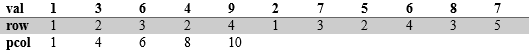
\includegraphics[width=0.8\linewidth]{figures/稀疏矩阵.png}
  \caption{矩阵 A 的 CSC 格式存储}
  \label{fig:4.1}
\end{figure}

\subsection{消去树}

稀疏 Cholesky 分解算法分为符号分析和数值分解两个阶段。在符号分析阶段,算法分析矩阵的非零模式,为后继的数值分解阶段做准备,使数值求解的时空复杂度都大幅下降;数值分解阶段将计算出分解的结果。与数值分解相比,符号分析的开销相对较小。

在整个算法中,消去树(elimination tree)是一个绕不开的概念,它指导了Cholesky分解的符号分析阶段,也为数值分解提供了一个基本框架。

形式上,$n$ 阶对称正定矩阵 $A=(a_{ij})$ 诱导出一个包含 $n$ 个节点的图 $G_A=(V_A, E_A)$,其中 $V_A=\{0,⋯,n-1\},E_A=\{(i,j)|0≤ j<i<n,  a_{ij}≠0\}$ 。

对于 Cholesky 分解 $A=LL^T, A=(a_{ij}), L=(l_{ij})$,有如下两个命题成立:

\begin{theorem}\label{theorem:1} 如果 $ a_{ij}\ne0 $,则 $l_{ij}\ne 0$。\end{theorem}
\begin{theorem}\label{theorem:2} 如果 $i<j<k$ 且  $l_{ji}\ne 0$,$l_{ki}\ne 0$,则 $l_{kj}\ne 0$ 。\end{theorem}

从定理 \ref{theorem:1} 可以知道,$L$ 继承了 $A$ 的所有非零模式。定理 \ref{theorem:2} 告诉我们,若在图 $G_L$ 中有 $(i, j)\in E_L$,则对所有 $k>j$ ,边 $(i, k)$ 实际上是冗余的,因为从节点 $i$ 可以途经 $j$ 到达 $k$。

由此可以对 $G_L$ 做剪枝,每个节点 $i$ 只需要维护至多一条出边 $(i,parent(i))$,其中 $parent(i)=\min(j:(i,j)\in E_L)$ ,这样得到的图称为矩阵 $A$ 的消去树。

\begin{figure}
  \centering
  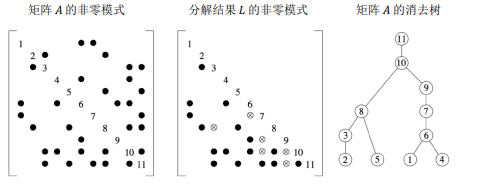
\includegraphics[width=0.8\linewidth]{figures/消去树.png}
  \caption{某矩阵的 Cholesky 分解和消去树}
  \label{fig:4.2}
\end{figure}

\subsection{符号分析}

在 Cholesky 分解过程中,矩阵 $L$ 在继承 $A$ 的所有非零模式基础上会增加一些新的非零元,称为填入元(fill-in)。图 \ref{fig:4.2} 中分解结果 $L$ 中的空心圈就是填入元。填入元会造成分解结果的稀疏性下降,进而提高算法的空间和时间复杂度。

在符号分解阶段,首先会寻找一个排列阵 $P$,称为减少填入排列,使得 $PAP^T$ 的分解结果中填入元尽量少。求最优减少填入排列是一个 NP 难问题,实践中一般采用启发式算法。

减少填入排列确定后,符号分析将对 $A$ 进行符号分解,计算出 $L$ 的非零模式,以消去树的形式给出。

\subsection{数值分解}

CHOLMOD 提供了两种数值求解方法,分别基于向上查看法和向左查看法。

向上查看法在每轮迭代中计算出矩阵 $L$ 的一行,因此也被称为行 Cholesky 算法。考虑等式 $A=LL^T$ 的如下分块:
\begin{equation}
\begin{bmatrix}
L_{11} & \\
l_{12}^T & l_{22}
\end{bmatrix}
\begin{bmatrix}
L_{11}^T & l_{12}\\
 & l_{22}
\end{bmatrix}=
\begin{bmatrix}
A_{11} & a_{12}\\
a_{12}^T & a_{22}
\end{bmatrix}
\end{equation}
其中 $l_{12}, a_{12}$ 为 $n-1$ 维向量; $l_{22}, a_{22}$ 为标量;$A_{11}$ 是原矩阵左上角的 $n-1$ 阶子矩阵,其 Cholesky 分解为 $L_{11}$。假设我们已经求出了前 $n-1$ 行的分解结果,即矩阵 $L_{11}$,则由分块矩阵乘法可得,
\begin{align}
l_{12}&=L_{11}/ a_{12}\\
a_{22}&=l_{12}^T l_{12}+l_{22}^2
\end{align}其中 “/” 符号表示求解三角方程组。

向上查看法的伪代码如算法 \ref{alg1} 所示,它在经过一些特别的优化后可用于稀疏矩阵的分解,当矩阵特别稀疏时,该方法比很多复杂方法更有效。

\begin{algorithm}
  \caption{向上查看Cholesky分解}
  \label{alg1}
  \small
  \begin{algorithmic}
  \REQUIRE 矩阵 $A$
  \ENSURE Cholesky 因子 $L$
  \FOR{k = 1 \TO n}
  \STATE $L_{k,1:k-1} \gets L_{1:k-1,1:k-1}/A_{1:k-1,k}$
  \STATE $L_{k,k} \gets \sqrt{A_{k,k} \minus L_{k,1:k-1} L_{k:1:k-1}^T} $  
  \ENDFOR
  \end{algorithmic}
\end{algorithm}

向左查看 Cholesky 分解算法在每轮迭代中计算出矩阵 $L$ 的一列,因此也被称为列 Cholesky 算法。在迭代进行至第 $k$ 轮时,考虑等式 $A=LL^T$ 的如下分块:
\begin{equation}
\begin{bmatrix}
L_{11} & &\\
l_{12}^T & l_{22} & \\
L_{31} & l_{32} & L_{33}
\end{bmatrix}
\begin{bmatrix}
L_{11}^T & l_{12} & L^T_{31}\\
 & l_{22} & l_{32}^T \\
 &  & L_{33}^T
\end{bmatrix}
=  \begin{bmatrix}
A_{11} & a_{12} & A_{31}^T\\
a_{12}^T & a_{22} &  a_{32}^T\\
A_{31} & a_{32} & A_{33}
\end{bmatrix}
\end{equation}
其中 $[L_{11};l_{12}^T;L_{31}]$ 是已经求出的前 $k-1$ 列,$[l_{22};l_{32}]$ 为待求列,$l_{22}$ 为标量。引入一个 $n-k+1$ 维的向量 $c$,根据分块矩阵乘法,可得待求列与已求列之间的关系:
\begin{align}
c &= \begin{bmatrix}
c_1 \\
c_2
\end{bmatrix} = 
\begin{bmatrix}
a_{22} \\
a_{32}
\end{bmatrix} - \begin{bmatrix}
l_{12}^T \\
L_{31}
\end{bmatrix}l_{12} \\
l_{22}&=\sqrt{c_1}\\
l_{32}&=c_2/l_{22}
\end{align}

根据这一递推关系,可以得到向左查看算法。这种算法能针对稀疏矩阵做多种优化。注意到,计算向量 $c$ 时,只需要考虑 $A$ 中的非零列,当我们分析出 $A$ 的非零元模式后,向量 $c$ 的计算效率将大大增加。向左查看法借助消去树的指导,可以分为很多子任务,更适合并行计算。向左查看法很容易改造为分块的版本,这构成了超节点(Supernodal)Cholesky 分解的基础。

\begin{algorithm}
  \caption{向左查看Cholesky分解}
  \label{alg2}
  \small
  \begin{algorithmic}
  \REQUIRE 矩阵 $A$
  \ENSURE Cholesky 因子 $L$
  \FOR{k = 1 \TO n}
  \STATE $c_{k:n}=A_{k:n,k}-L_{k:n,1:k-1} L_{k,1:k-1}^T$
  \STATE $L_{k,k}=\sqrt{c_k}$
  \STATE $L_{k+1:n,k}=c_{k+1:n,k}/L_{k,k}$
  \ENDFOR
  \end{algorithmic}
\end{algorithm}

\section{程序实现}

程序实现主要分为两步,调用 CPP2PY 自动生成代码,并在此基础上进行二次开发。

CHOLMOD\cite{chen2008algorithm, davis2008user} 库完成 Cholesky 分解需要调用的例程主要有两个:\lstinline{cholmod_analyze} 和 \lstinline{cholmod_factorize},前者进行符号分析,后者完成数值分解。调用 \lstinline{cholmod_analyze} 时需要给出寻找减小填入排列和数值分解的方法。

CHOLMOD 主要提供了两种计算减填序列的方法,近似最小度数法(Approximate Minimum Degree)和嵌套分割方法(Nested dissection),METIS 是后者的一个实现。受支持的数值分解方法有两种:simplicial(基于向上查看法)和 supernodal(基于向左查看的超节点法)。\lstinline{cholmod_analyze} 根据选择的数值分解算法返回不同的符号分析结果。

减少填入排列和分解方法都选定后,\lstinline{cholmod_analyze} 例程被调用,返回一个 \lstinline{cholmod_factor} 结构体,该结构作为 \lstinline{cholmod_factorize} 的输入,指导后者进行数值分解。

CPP2PY 能正确地解析 CHOLMOD 库的源程序,但考虑到算法库体量庞大,包含了上百个 API 接口,其中与 Cholesky 分解直接相关的只有十多个,直接解析源程序将生成大量无关代码。为了后续开发的方便,可以将源程序头文件中有用的部分手动提取出来,让 CPP2PY 只解析这部分子集。为了处理泛型指针 \lstinline{void*} ,需要编写类型转换器子类,根据属性名指定泛型指针的实际类型。

\begin{algorithm}
  \caption{将 \lstinline$scipy.sparse$ 稀疏矩阵转换为 \lstinline$cholmod_sparse$}
  \label{alg3}
  \small
  \begin{algorithmic}
  \REQUIRE \lstinline$scipy.sparse$ 矩阵 $m$
  \ENSURE \lstinline$cholmod_sparse$ 矩阵 $out$
  \IF{not m.iscsc()}
    \STATE m = m.tocsc()
  \ENDIF
  \STATE 根据 $m$ 中的数据,初始化 $out$
  \RETURN $out$
  \end{algorithmic}
\end{algorithm}


\begin{algorithm}
  \caption{将 \lstinline$cholmod_sparse$ 稀疏矩阵转换为 \lstinline$scipy.sparse$}
  \label{alg4}
  \small
  \begin{algorithmic}
  \REQUIRE \lstinline$cholmod_sparse$ 矩阵 $m$
  \ENSURE \lstinline$scipy.sparse$ 矩阵 $out$
  \STATE 根据 $m$ 中的数据,调用 NumPy C API,初始化 $out$ 对象
  \STATE 为 $out$ 重写析构函数,保证 $out$ 被析构时内存被正确释放
  \RETURN $out$
  \end{algorithmic}
\end{algorithm}

CHOLMOD 根据不同的数据结构和上下文提供了分配、回收内存的多个例程,CPP2PY 不知道该如何调用这些例程。二次开发中需要手动处理内存释放问题。

类型转换是跨语言接口的关键部分。\lstinline{scipy.sparse} 模块定义了多种稀疏矩阵类,而 CHOLMOD 使用的稀疏矩阵 \lstinline{cholmod_sparse} 以 CSC 格式存储。为了让封装后的CHOLMOD能分解 \lstinline{scipy.sparse} 稀疏矩阵,要实现后者与 \lstinline{cholmod_sparse} 之间的相互转换。伪代码如算法 \ref{alg3} 和 \ref{alg4} 所示,实现中尽可能避免了大块数据的复制和移动,从而保证了类型转换的效率。

封装后的Cholesky分解算法伪代码如算法 \ref{alg5} 所示。

\begin{algorithm}
  \caption{稀疏Cholesky分解Python接口}
  \label{alg5}
  \small
  \begin{algorithmic}
  \REQUIRE \lstinline$scipy.sparse$ 矩阵 $A$,分解模式 mode,排序方法 ordering\_method
  \ENSURE \lstinline$scipy.sparse$ 格式的 Cholesky 因子 $L$
  \STATE 将 $A$ 转换为 \lstinline$cholmod_sparse$ 稀疏矩阵 $m$
  \STATE 初始化参数
  \STATE 调用 \lstinline$cholmod_analyze$ 进行符号分析,得到 $factor$
  \STATE 调用 \lstinline$cholmod_factorize$ 分解 $factor$
  \STATE 将 $factor$ 转换为 \lstinline$scipy.sparse$ 稀疏矩阵 $L$
  \RETURN $L$
  \end{algorithmic}
\end{algorithm}

\section{实验测试}

\subsection{实验设置}

实验的系统环境 Ubuntu 20.04,CPU 为 AMD(R) RYZEN(TM) 5800H,SuiteSparse 版本为 5.7.1,CHOLMOD 版本为 3.0.14,Python 和 SciPy 的版本分别为 3.8.10 和 1.6.3。实验以直接用 C 语言调用 CHOLMOD 为基线,验证调用 Python 接口分解稀疏矩阵的结果是否与之一致,并比较二者的性能。

为了规避 OS 调度等因素的影响,性能测试的标准为多次运行取最优。Cholesky 分解策略指定为以下四种:Simplicial/AMD、Simplicial/METIS、Supernodal/AMD、Supernodal/METIS。这些策略的详细含义见上一节。

\begin{table}
  \centering
  \caption{测例矩阵}
  \begin{tabular}{lll}
    \toprule
     测例           &  行/列数  &  下三角非零元数 \\
    \midrule
     ted\_B          &  10605    &  77592          \\
     s3rmt3m3       &  5357     &  106526         \\
     thermomech\_dM  &  204316   &  813716         \\
     parabolic\_fem  &  525825   &  2100225        \\
     nd12k          &  36000    &  7128473        \\
     nd24k          &  72000    &  14393817       \\
     PFlow\_742      &  742793   &  18940627       \\
     boneS10        &  914898   &  28191660       \\
    \bottomrule
  \end{tabular}
  \label{tab:4.1}
\end{table}


实验测试数据\footnote{数据来源于 \url{https://sparse.tamu.edu/}.}罗列如表 \ref{tab:4.1},它们均为对称正定矩阵。这些矩阵规模庞大,只能以稀疏形式存储。图 \ref{fig:4.3} 展示了它们的非零元模式。


\begin{figure}
  \centering
  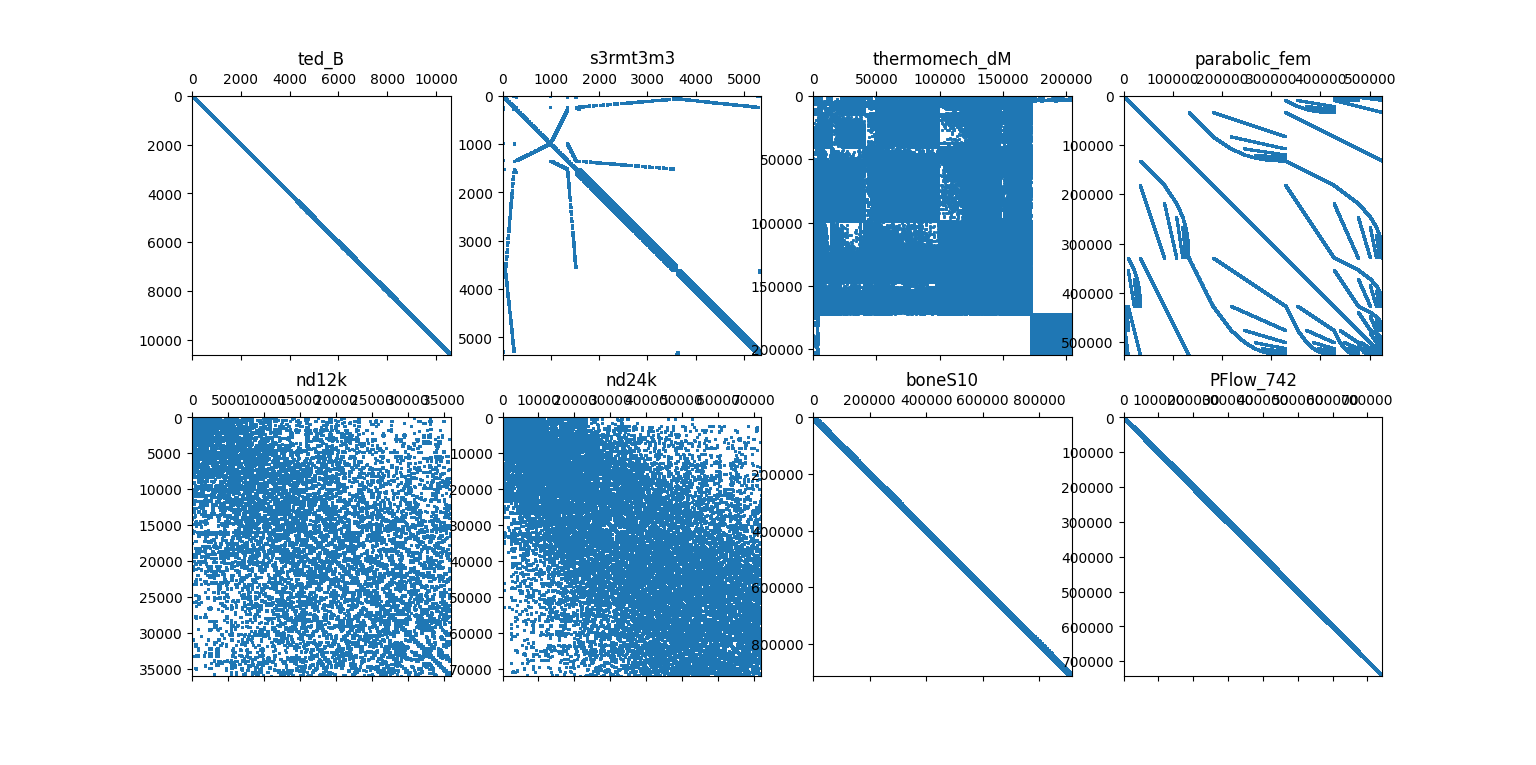
\includegraphics[width=\linewidth]{figures/测例矩阵.png}
  \caption{测例矩阵的非零元模式}
  \label{fig:4.3}
\end{figure}

\subsection{实验结果}

调用 Python 接口的分解结果与直接编写 C 程序得到的结果在误差范围内一致,确保了实验的正确性。

由表 \ref{tab:4.21} 可知,与直接以 C 语言编程相比,调用 Python 接口进行分解花费的额外时间占原耗时比例通常在 5\% 以内。性能测试的原始数据见附录表 \ref{tab:4.2} 和 \ref{tab:4.3}。

\begin{table}
  \centering
  \caption{Python 接口相对 C 的额外开销占原耗时比例}
  \begin{tabular}{lllll}
    \toprule
     测例           &  Simplicial/AMD  &  Simplicial/METIS  &  Supernodal/AMD  &  Supernodal/METIS \\
    \midrule
    ted\_B & 2.01\% & 4.35\% & 2.24\% & 8.47\% \\
 s3rmt3m3       &        0.50\% & 4.39\% & 4.88\% & 6.04\% \\
thermomech\_dM  &        0.33\% & 0.02\% & 0.25\% & 5.31\% \\
parabolic\_fem  &        0.09\% & 0.99\% & 1.83\% & 1.36\% \\
nd12k          &         0.06\% & 0.26\% & 0.66\% & 0.16\% \\
nd24k          &       0.14\% & 0.50\% & 0.09\% & 0.09\% \\
PFlow\_742      &        0.01\% & 0.05\% & 0.23\% & 0.32\% \\
boneS10        &        0.11\% & 0.24\% & 0.31\% & 0.66\% \\
    \bottomrule
  \end{tabular}
  \label{tab:4.21}
\end{table}

% !TeX root = ../thuthesis-example.tex

\chapter{总结}

本文设计并实现了一种从 C/C++ 声明自动构建 Cython 包装代码的开发工具,即 CPP2PY。该工具能以有效降低 Cython 语言的学习成本,减少用 Cython 编写 C/C++ 扩展模块时的重复性工作,提高 FFI 开发的生产力。

CPP2PY 接受 C/C++ 头文件为输入,输出接口的 Cython 包装代码、构建脚本和对应 Python 类型注解。本项目经过了详尽的软件测试,覆盖率达到 93 \%。受支持的 C/C++ 语法特性包括函数、全局变量、宏、枚举、类、结构体、联合、类的继承和多态、默认参数、重载、类型别名、异常等。CPP2PY 能处理相当一部分类型在 C++ 和 Python 之间的自动转换,包括基本数值类型及其指针、字符串、部分 STL 容器、枚举、类及其指针等。它还提供了可扩展的自动类型转换模块,只要用户重写转换器基类,指明特定类型数据的转换方法,就能让 CPP2PY 支持新的数据类型。 

基于 CPP2PY,本文封装了 SuiteSpars CHOLMOD 中的大规模稀疏矩阵Cholesky分解模块,为Python科学计算库SciPy实现了正确而高效的稀疏矩阵分解算法,弥补了SciPy和NumPy没有稀疏矩阵Cholesky分解功能的缺憾。封装后的接口与原 C 函数库相比性能损失低于5\%。高性能来源于高度优化的 Cython 编译器,以及类型转换实现中直接操纵指针,避免了整块内存的复制。

C++ 的语法变化复杂,作为一个自动构建工具,CPP2PY 还有诸多未竟之处。未来工作的主要落脚点在两个方面。

首先是支持更多的 C++ 特性。除了第三章中提到的限制之外,CPP2PY 不支持 C++ 模板相关的语法。在 Python 中,并没有与模板对应的语法。但是只要指定模板参数的类型,就能以封装普通类的方式封装模板类。实现模板功能的关键之一在于类型系统,目前 CPP2PY 的类型系统完全基于 libclang,不足以支持模板参数的替换。

其次是支持更多的数据类型,包括函数指针、智能指针等。将 Python 函数对象直接转换成 C 函数指针是不可能的,更合理的做法可能是允许用户将其它 C 函数当作函数指针使用;支持智能指针的难点在于,各种指针类型管理所有权的方式难以相互兼容,指针对象的所有权问题也许只能手动解决。

不得不说,即使是像 SWIG 这样成熟的 FFI 自动构建工具,其能力范围也是有限的。一旦用户的需求超出了这种限度,就不得不开始受工具本身掣肘。需要封装的 C/C++ 程序越复杂,自动生成的接口就越难以使用。相比之下,基于 Cython 语言的 CPP2PY 能提供二次开发的更多可能,尽管同时也带来了 Cython 语法的限制。

% 其他部分
\backmatter

% 插图和附表清单
% 本科生的插图索引和表格索引需要移至正文之后、参考文献前
% \listoffiguresandtables  % 插图和附表清单(仅限研究生)
\listoffigures           % 插图清单
\listoftables            % 附表清单

% 参考文献
\bibliography{ref/refs}  % 参考文献使用 BibTeX 编译
% \printbibliography       % 参考文献使用 BibLaTeX 编译

% 附录
% 本科生需要将附录放到声明之后,个人简历之前
\appendix
% \input{data/appendix-survey}       % 本科生:外文资料的调研阅读报告
% !TeX root = ../thuthesis-example.tex

\begin{translation}
\label{cha:translation}

\title{Cython 教程:使用 C 库}
\maketitle

\tableofcontents


除了编写高效代码之外,Cython的主要用途之一是从Python代码调用外部C库。由于Cython本身可以编译为 C 代码,在代码中直接调用C函数实际上很容易。下面给出了一个在Cython代码中使用和包装外部C库的完整例子,包括适当的错误处理,以及为Python和Cython代码设计合适API时的注意事项。

设想一下,你需要一种有效的方法在 FIFO 队列中存储整数值。因为内存真的很重要,而值实际上来自C代码,所以你无法不能在 \lstinline{list} 或 \lstinline{deque} 中创建存储Python \lstinline{int} 对象。你想要寻找 C 语言中的队列实现。

在互联网上经过一番搜索,你找到了 C 算法库 CAlg\footnote{Simon Howard, C Algorithms library, http://c-algorithms.sourceforge.net/},决定使用其双端队列。然而,为了使处理更容易,你决定把它包装在一个可以封装所有内存管理的Python扩展类型中。

\section{定义外部声明}
队列实现的C语言API定义在头文件 \lstinline{c-algorithms/src/queue.h} 中,大致上是这样的:

\begin{framed}
\begin{lstlisting}[language=c]
/* queue.h */

typedef struct _Queue Queue;
typedef void *QueueValue;

Queue *queue_new(void);
void queue_free(Queue *queue);

int queue_push_head(Queue *queue, QueueValue data);
QueueValue queue_pop_head(Queue *queue);
QueueValue queue_peek_head(Queue *queue);

int queue_push_tail(Queue *queue, QueueValue data);
QueueValue queue_pop_tail(Queue *queue);
QueueValue queue_peek_tail(Queue *queue);

int queue_is_empty(Queue *queue);
\end{lstlisting}    
\end{framed}


要实现目标,第一步是在一个 \lstinline{.pxd} 文件中重新定义C语言的API,例如 \lstinline{cqueue.pxd}:

\begin{framed}
\begin{lstlisting}[language=python]
cdef extern from "c-algorithms/src/queue.h":
    ctypedef struct Queue:
        pass
    ctypedef void* QueueValue

    Queue* queue_new()
    void queue_free(Queue* queue)

    int queue_push_head(Queue* queue, QueueValue data)
    QueueValue  queue_pop_head(Queue* queue)
    QueueValue queue_peek_head(Queue* queue)

    int queue_push_tail(Queue* queue, QueueValue data)
    QueueValue queue_pop_tail(Queue* queue)
    QueueValue queue_peek_tail(Queue* queue)

    bint queue_is_empty(Queue* queue)
\end{lstlisting}
\end{framed}

请注意,这些声明与头文件的声明几乎是一样的,所以你常常可以直接把它们复制过来。然而,你不需要提供所有的声明,只需要提供那些你在代码或其他声明中使用的声明,这样Cython就能看到一个足够的、一致的子集。然后,考虑对它们进行一定程度的调整,使它们在Cython中工作得更舒适。

具体来说,你应该注意为C函数选择适当的参数名,因为Cython允许你以关键字传递参数。以后再改变它们是一种向后不兼容的API修改。现在就选择好的参数名会使在Cython代码中的使用这些函数更愉快。

Cython 声明与我们上面的头文件有一个值得注意的区别,那就是第一行对 \lstinline{Queue} 结构体的声明。 \lstinline{Queue} 被视作一个不透明的句柄,只有被调用的库才知道里面到底是什么。既然没有Cython代码需要知道这个结构的内容,我们就不需要声明它的内容,只提供一个空的定义(因为我们不想声明C文件中引用的 \lstinline{_Queue} 类型)。 

\lstinline{cdef struct Queue: pass} 和 \lstinline{ctypedef struct Queue: pass} 之间有一个微妙的区别。前者声明了一个类型,在C语言代码中被引用为 \lstinline{struct Queue},而后者在C语言中被引用为 \lstinline{Queue}。这是C语言的一个特色,Cython无法隐藏。大多数现代C语言库都使用 \lstinline{ctypedef} 这种结构。

另一个区别在最后一行,\lstinline{queue_is_empty()} 函数的整数返回值实际上是一个C布尔值,也就是说,唯一有趣的地方是它是否为零,表示队列是否为空。这最好由Cython的 \lstinline{bint} 类型来表达,当在C语言中使用时,它是一个普通的 \lstinline{int} 类型,但当转换为Python对象时,它被映射为Python的布尔值 \lstinline{True} 和 \lstinline{False}。这种在 \lstinline{.pxd} 文件中严格声明的方式通常可以简化使用它们的代码。

为每个你使用的库,甚至每个头文件(或功能组)定义一个 \lstinline{.pxd} 文件是很好的做法,如果API数目很大的话。这样可以简化它们在其他项目中的重用。有时,你可能需要使用标准库中的C函数,或者想从CPython直接调用C-API。对于这样的常见需求,Cython提供了一组标准的 \lstinline{.pxd} 文件,以一种随时可用的、Cython 化的方式提供这些声明。主要的包是 \lstinline{cpython}、\lstinline{libc} 和 \lstinline{libcpp}。NumPy库也有一个标准的 \lstinline{.pxd} 文件 \lstinline{numpy},因为该库在Cython代码中经常被使用。\lstinline{.pxd} 文件的完整列表参见Cython的 \lstinline{Cython/Includes/} 源代码。

\section{编写一个包装类}

声明了我们的C语言库的API之后,我们可以开始设计Queue类,用于包装 C 语言队列。它将存在于一个名为 \lstinline{queue.pyx}/\lstinline{queue.py} 的文件中。

注意,\lstinline{.pyx}/\lstinline{.py} 文件的名称必须与带有C库的声明的 \lstinline{cqueue.pxd} 文件不同,因为两者描述的代码不同。与 \lstinline{.pyx}/\lstinline{.py} 文件同名的 \lstinline{.pxd} 文件定义了前者代码的导出声明。由于 \lstinline{cqueue.pxd} 文件包含了 C 语言库的声明,所以不能有一个 \lstinline{.pyx}/\lstinline{.py} 文件与之同名,否则 Cython 会将他们关联在一起。

这是编写 \lstinline{Queue} 类的第一步:

\begin{framed}
\begin{lstlisting}[language=python]
cimport cqueue


cdef class Queue:
    cdef cqueue.Queue* _c_queue

    def __cinit__(self):
        self._c_queue = cqueue.queue_new()
\end{lstlisting}
\end{framed}

注意定义的是 \lstinline{__cinit__} 而不是 \lstinline{__init__}。虽然 \lstinline{__init__} 也是可用的,但它不能保证可以运行(例如,用户可以创建一个子类,但却忘记调用基类的构造函数)。考虑到不初始化 C 指针经常导致Python解释器的硬崩溃,Cython提供了 \lstinline{__cinit__},它总是在构造时立即被调用,甚至在 CPython 调用 \lstinline{__init__} 之前,因此它是初始化新实例的静态属性(\lstinline{cdef} 字段)的正确地方。然而,由于 \lstinline{__cinit__} 是在对象构造过程中调用的,所以 \lstinline{self} 还没有完全构造好,我们必须避免对 \lstinline{self} 做任何事情,除了赋值给静态属性(\lstinline{cdef} 字段)。

还要注意的是,上述方法不需要参数,尽管子类型可能希望接受一些参数。无参数的 \lstinline{__cinit__()} 方法是这里的一个特例,它只是不接受任何传递给构造函数的参数,并不阻止子类添加参数。如果在 \lstinline{__cinit__()} 的签名中使用了参数,则必须与类层次结构中任何的 \lstinline{__init__} 方法的参数一致。

\section{内存管理}

在我们继续实现其他方法之前,有必要指出上一节的实现并不安全。如果在调用 \lstinline{queue_new()} 时出现任何错误,这段代码将简单地隐藏错误,程序可能会在之后的某处崩溃。根据 \lstinline{queue_new()} 函数的文档,调用失败的唯一原因是内存不足。在这种情况下,它将返回 \lstinline{NULL},而不是一个指向新队列的指针。

解决此问题的Python方法是引发 \lstinline{MemoryError} 异常。我们可以这样修改初始化函数:

\begin{framed}
\begin{lstlisting}[language=python]
cimport cqueue


cdef class Queue:
    cdef cqueue.Queue* _c_queue

    def __cinit__(self):
        self._c_queue = cqueue.queue_new()
        if self._c_queue is NULL:
            raise MemoryError()
\end{lstlisting}
\end{framed}

在特定情况下,创建并抛出一个新的异常实例 \lstinline{MemoryError} 实际上可能会失败,因为我们正在耗尽内存。幸运的是,CPython提供了一个C-API函数\lstinline{ PyErr_NoMemory() },它可以安全地为我们引发正确的异常。每当你编写\lstinline{ raise MemoryError }或\lstinline{ raise MemoryError() }时,Cython会自动替换将它这个C-API调用。如果使用旧版本 Cython,则必须从标准包\lstinline{ cpython }中cimport C-API函数并调用。 

接下来要做的事情是,在Queue实例不再被使用时(即它的所有引用被删除)时进行清理。为此,CPython 提供了一个回调函数,Cython将其作为特殊方法 \lstinline{__dealloc__()} 提供。在我们的例子中,要做的就是释放C队列,当然前提是我们成功地在 \lstinline{__cinit__} 中初始化了它:

\begin{framed}
\begin{lstlisting}[language=python]
def __dealloc__(self):
    if self._c_queue is not NULL:
        cqueue.queue_free(self._c_queue)
\end{lstlisting}
\end{framed}

\section{编译链接}

现在,我们有了一个可以工作的Cython模块,我们可以测试这个模块。要编译它,我们需要为setuptools配置一个\lstinline{ setup.py }脚本。下面是用于编译Cython模块的最基本脚本:

\begin{framed}
\begin{lstlisting}[language=python]
from setuptools import Extension, setup
from Cython.Build import cythonize

setup(
    ext_modules = cythonize([Extension("queue", ["queue.pyx"])])
)
\end{lstlisting}
\end{framed}

要针对外部C库进行构建,我们需要确保Cython找到必要的库。有两种实现方法。第一,我们可以告诉setuptools在哪里找到c源文件,让它来自动编译\lstinline{ queue.c }实现。或者,我们可以构建并安装C-Alg作为系统库,并动态链接它。如果其他应用程序也使用C-Alg,则后者很有用。

\subsection{静态链接}

为了自动构建 C 代码,我们需要在 \lstinline{queue.pyx}/\lstinline{queue.py} 中包含下列编译指令,

\begin{framed}
\begin{lstlisting}[language=python]
# distutils: sources = c-algorithms/src/queue.c
# distutils: include_dirs = c-algorithms/src/

cimport cqueue


cdef class Queue:
    cdef cqueue.Queue* _c_queue

    def __cinit__(self):
        self._c_queue = cqueue.queue_new()
        if self._c_queue is NULL:
            raise MemoryError()

    def __dealloc__(self):
        if self._c_queue is not NULL:
            cqueue.queue_free(self._c_queue)
\end{lstlisting}
\end{framed}

\lstinline{sources }编译指令给出了setuptools将要编译并(静态地)链接到最终扩展模块的C文件路径。一般来说,所有相关头文件都应该在\lstinline{ include_dirs }中找到。现在我们可以使用以下命令来构建项目:

\begin{framed}
\begin{lstlisting}[language=sh]
$ python setup.py build_ext -i
\end{lstlisting}
\end{framed}
测试构建是否成功,

\begin{framed}
\begin{lstlisting}[language=sh]
$ python -c 'import queue; Q = queue.Queue()'
\end{lstlisting}
\end{framed}

\subsection{动态链接}

如果我们要包装的库已经安装在系统上,那么动态链接是有用的。要执行动态链接,我们首先需要构建和安装c-alg。

\begin{framed}
\begin{lstlisting}[language=sh]
$ cd c-algorithms
$ sh autogen.sh
$ ./configure
$ make install
\end{lstlisting}
\end{framed}

此后应该存在文件 \lstinline{/usr/local/lib/libcalg.so}。

此路径适用于Linux系统,可能在其他平台上有所不同,所以你需要根据 \lstinline{libcalg.so} 还是 \lstinline{libcalg.dll} 存在于在你的系统上来修改接下来的教程。

在这种方法中,我们需要告诉安装脚本链接外部库。为此,我们需要扩展安装脚本,将扩展设置从

\begin{framed}
\begin{lstlisting}[language=python]
ext_modules = cythonize([Extension("queue", ["queue.pyx"])])
\end{lstlisting} 
\end{framed}
更改为
\begin{framed}
\begin{lstlisting}[language=python]
ext_modules = cythonize([
    Extension("queue", ["queue.pyx"],
              libraries=["calg"])
    ])
\end{lstlisting}
\end{framed}

现在我们应该能这样构建项目,
\begin{framed}
\begin{lstlisting}[language=sh]
$ python setup.py build_ext -i
\end{lstlisting}
\end{framed}

如果 \lstinline{libcalg} 被安装到其它位置,用户可以通过从外部传递适当的C编译器标志来提供所需的参数,例如:

\begin{framed}
\begin{lstlisting}[language=sh]
CFLAGS="-I/usr/local/otherdir/calg/include"  \
LDFLAGS="-L/usr/local/otherdir/calg/lib"     \
    python setup.py build_ext -i
\end{lstlisting}
\end{framed}

在运行我们的模块之前,我们还需要保证 \lstinline{libcalg} 的路径在 \lstinline{LD_LIBRARY_PATH} 环境变量中,通过设置:

\begin{framed}
\begin{lstlisting}[language=sh]
$ export LD_LIBRARY_PATH=$LD_LIBRARY_PATH:/usr/local/lib
\end{lstlisting}
\end{framed}

在第一次编译了模块后,我们可以导入它,并实例化一个新的 \lstinline{Queue}:

\begin{framed}
\begin{lstlisting}[language=sh]
$ export PYTHONPATH=.
$ python -c 'import queue; Q = queue.Queue()'
\end{lstlisting}
\end{framed}

然而,这是我们的 \lstinline{Queue} 类到目前为止所能做的全部工作,让我们来使它更有用。

\section{功能映射}

在实现这个类的公共接口之前,最好看看Python提供了哪些接口,例如它的 \lstinline{list} 或 \lstinline{collections.deque} 类。由于我们只需要一个先进先出的队列,提供 \lstinline{append()}、\lstinline{peek()} 和 \lstinline{pop()} 方法就足够了,另外还有一个 \lstinline{extend()} 方法可以一次添加多个值。另外,由于我们已经知道所有的值都将来自C语言,所以现在最好只提供 \lstinline{cdef} 方法,并直接给它们一个C语言接口。

在C语言数据结构中,常常以 \lstinline{void*} 的方式存储任意类型的数据。由于我们只想存储 \lstinline{int} 值,而它的大小通常与指针类型的大小相同,可以通过一个技巧来避免额外的内存分配:我们把 \lstinline{int} 转换成 \lstinline{void*},直接存储为指针值,反之亦然。

下面是 \lstinline{append()} 方法的一个简单实现:

\begin{framed}
\begin{lstlisting}[language=python]
cdef append(self, int value):
    cqueue.queue_push_tail(self._c_queue, <void*>value)
\end{lstlisting}
\end{framed}

同样,与 \lstinline{__cinit__()} 方法相同的错误处理考虑也适用于此,因此我们最终用这个实现代替:

\begin{framed}
\begin{lstlisting}[language=python]
cdef append(self, int value):
    if not cqueue.queue_push_tail(self._c_queue,
                                  <void*>value):
        raise MemoryError()
\end{lstlisting}
\end{framed}

增加一个 \lstinline{extend()} 方法现在应该很直接:

\begin{framed}
\begin{lstlisting}[language=python]
cdef extend(self, int* values, size_t count):
    """Append all ints to the queue.
    """
    cdef int value
    for value in values[:count]:
        self.append(value)
\end{lstlisting}
\end{framed}这样从 C 语言中读取值很方便。

到目前为止,我们只能向队列中添加数据。下一步是编写两个方法来获取第一个元素:\lstinline{peek()} 和 \lstinline{pop()},它们分别提供只读和破坏性的读访问。为了避免在将 \lstinline{void*} 直接转换为 \lstinline{int} 时出现编译器警告,我们使用了一个足够大的中间数据类型来容纳 \lstinline{void*}。这里使用 \lstinline{Py_ssize_t}:

\begin{framed}
\begin{lstlisting}[language=python]
cdef int peek(self):
    return <Py_ssize_t>cqueue.queue_peek_head(self._c_queue)

cdef int pop(self):
    return <Py_ssize_t>cqueue.queue_pop_head(self._c_queue)
\end{lstlisting}
\end{framed}

通常,在C语言中,当我们将一个较大的整数类型转换为较小的整数类型而不检查边界时,会有丢失数据的风险,而 \lstinline{Py_ssize_t} 可能是一个比 \lstinline{int} 更大的类型。但是由于我们控制了如何将值添加到队列中,我们已经知道所有在队列中的值都适用于 \lstinline{int},所以上面从 \lstinline{void*} 到 \lstinline{Py_ssize_t} 到 \lstinline{int}(返回类型)的转换在设计上是安全的。

\section{错误处理}

现在,当队列为空时会发生什么?根据文档,这些函数返回一个 \lstinline{NULL} 指针,这通常不是一个有效值。但是,由于我们只是简单地对整数进行转换,我们不能再区分返回值为 \lstinline{NULL} 是由于队列为空,还是因为队列中存储的值是 \lstinline{0}。在Cython代码中,我们希望第一种情况引发一个异常,而第二种情况应该简单地返回 "0"。为了处理这个问题,我们需要对这个值进行特殊处理,并检查队列是否确实是空的。

\begin{framed}
\begin{lstlisting}[language=python]
cdef int peek(self) except? -1:
    cdef int value = <Py_ssize_t>cqueue.queue_peek_head(self._c_queue)
    if value == 0:
        if cqueue.queue_is_empty(self._c_queue):
            raise IndexError("Queue is empty")
    return value
\end{lstlisting}
\end{framed}

请注意我们是如何在方法返回值通常不是 0 的情况下,有效地创建了一条捷径的——只有特殊情况需要额外检查队列是否为空。

方法签名中的 \lstinline{except? -1} 声明也属于同一类别。如果这个函数是一个返回Python对象值的Python函数,CPython会简单地在内部返回 \lstinline{NULL} 而不是Python对象来表示异常,这将立即被周围的代码所传播。

问题是返回类型是 \lstinline{int},任何 \lstinline{int} 值都是有效的队列元素值,所以没有办法显式地向调用代码发出错误信号。事实上,没有这样的声明,Cython就没有明确的办法知道在异常情况下应该返回什么,也没有办法让调用代码知道这个方法可能以异常退出。调用代码处理这种情况的唯一方法是在从函数返回时调用 \lstinline{PyErr_Occurred()} 来检查是否有异常被抛出,如果有,就传播异常。这显然对性能有影响。因此,Cython允许你声明在异常情况下应该隐式返回哪个值,这样周围的代码只需要接收到这个确切的值时检查异常。

我们选择使用 -1作为异常返回值,因为我们希望它是一个不太可能被放入队列的值。\lstinline{except? -1} 声明表明返回值是模糊的(毕竟队列中可能有值为 -1),在调用代码中需要使用 \lstinline{PyErr_Occurred()} 进行额外的异常检查。如果没有它,调用这个方法并收到异常返回值的 Cython 代码会默认(有时会错误地)已经产生了一个异常。而所有其他的返回值在任何情况都几乎不带来任何性能损失,从而再次为"正常"值创造了一个捷径。

既然 \lstinline{peek()} 方法已经实现,\lstinline{pop()} 方法也需要调整。因为它从队列中移除一个值,然而,仅仅测试弹出元素后队列是否为空是不够的。相反,我们必须在弹出前测试它。

\begin{framed}
\begin{lstlisting}[language=python]
cdef int pop(self) except? -1:
    if cqueue.queue_is_empty(self._c_queue):
        raise IndexError("Queue is empty")
    return <Py_ssize_t>cqueue.queue_pop_head(self._c_queue)
\end{lstlisting}异常传播的返回值与 \lstinline{peek()} 的声明完全一致。
\end{framed}

最后,我们可以通过实现\lstinline{__bool__()}特殊方法,以Python的惯用方式为队列提供一个空闲指示器(注意Python 2称这个方法为\lstinline{__nonzero__},而Cython支持使用这两个名字)。

\begin{framed}
\begin{lstlisting}[language=python]
def __bool__(self):
    return not cqueue.queue_is_empty(self._c_queue)
\end{lstlisting}
\end{framed}

注意,该方法返回 \lstinline{True} 或 \lstinline{False},因为我们在 \lstinline{cqueue.pxd} 中声明 \lstinline{queue_is_empty()} 函数的返回类型为 \lstinline{bint}。

\appendix


% 书面翻译的参考文献
% \bibliographystyle{unsrtnat}
% \bibliography{ref/appendix}

% 书面翻译对应的原文索引
\begin{translation-index}
  \nocite{usingc}
  \bibliographystyle{unsrtnat}
  \bibliography{ref/appendix}
\end{translation-index}

\end{translation}
  % 本科生:外文资料的书面翻译
% !TeX root = ../thuthesis-example.tex

\chapter{补充内容}


\begin{table}
  \centering
  \caption{C 接口性能测试结果(单位:秒)}
  \begin{tabular}{lllll}
    \toprule
     测例           &  Simplicial/AMD  &  Simplicial/METIS  &  Supernodal/AMD  &  Supernodal/METIS \\
    \midrule
     ted\_B          &  0.002981        &  0.009287          &  0.006036        &  0.012391         \\
     s3rmt3m3       &  0.020771        &  0.025399          &  0.015166        &  0.018996         \\
     thermomech\_dM  &  0.495037        &  1.063929          &  0.472786        &  1.07442          \\
     parabolic\_fem  &  7.374794        &  4.944353          &  4.218062        &  3.915948         \\
     nd12k          &  324.664         &  173.5749          &  265.0318        &  132.3255         \\
     nd24k          &  1692.008        &  666.9054          &  1463.497        &  574.2366         \\
     PFlow\_742      &  1788.484        &  458.3058          &  1419.988        &  325.8464         \\
     boneS10        &  225.0506        &  104.5306          &  146.6788        &  67.43623         \\
    \bottomrule
  \end{tabular}
  \label{tab:4.2}
\end{table}

\begin{table}
  \centering
  \caption{Python 接口性能测试结果(单位:秒)}
  \begin{tabular}{l llll}
    \toprule
     测例           &  Simplicial/AMD  &  Simplicial/METIS  &  Supernodal/AMD  &  Supernodal/METIS \\
    \midrule
     ted\_B          &  0.003041        &  0.009691          &  0.006171        &  0.01344          \\
     s3rmt3m3       &  0.020667        &  0.026513          &  0.015906        &  0.020143         \\
     thermomech\_dM  &  0.496656        &  1.064099          &  0.471594        &  1.131495         \\
     parabolic\_fem  &  7.381092        &  4.993541          &  4.295058        &  3.969384         \\
     nd12k          &  324.4743        &  174.0312          &  266.7832        &  132.5375         \\
     nd24k          &  1694.357        &  670.2118          &  1462.218        &  574.7287         \\
     PFlow\_742      &  1788.709        &  458.5141          &  1423.285        &  326.8807         \\
     boneS10        &  225.2972        &  104.7782          &  147.1279        &  67.88306         \\
    \bottomrule
  \end{tabular}
  \label{tab:4.3}
\end{table}

% 致谢
\input{data/acknowledgements}

% 声明
\statement
% 将签字扫描后的声明文件 scan-statement.pdf 替换原始页面
% \statement[file=scan-statement.pdf]
% 本科生编译生成的声明页默认不加页脚,插入扫描版时再补上;
% 研究生编译生成时有页眉页脚,插入扫描版时不再重复。
% 也可以手动控制是否加页眉页脚
% \statement[page-style=empty]
% \statement[file=scan-statement.pdf, page-style=plain]

% 个人简历、在学期间完成的相关学术成果
% 本科生可以附个人简历,也可以不附个人简历
% \input{data/resume}

% 指导教师/指导小组学术评语
% 本科生不需要
\input{data/comments}

% 答辩委员会决议书
% 本科生不需要
\input{data/resolution}

% 本科生的综合论文训练记录表(扫描版)
% \record{file=scan-record.pdf}

\end{document}
